\documentclass[12pt]{report}
\usepackage{amsmath}
\usepackage{setspace}
\usepackage{mathrsfs}

\makeatletter
\newif\if@restonecol
\makeatother
\let\algorithm\relax

\newcommand{\lsp}[1]{\large\renewcommand{\baselinestretch}{#1}\normalsize}
\lsp{1.5}

\def\theend{\hspace*{\fill}\rule{0.8ex}{0.8ex}\vspace*{0.8ex}}
\def\theupend{\vspace*{-0.6cm}\hspace*{\fill}\rule{0.8ex}{0.8ex}\vspace*{0.8ex}}
\def\mund#1{{\smallskip\noindent{\bf #1}}}
\def\proof{}

%\newcommand{\eat}[1]{}
%\let\endalgorithm\relax
\usepackage[lined,boxed,vlined,ruled]{algorithm2e}

\usepackage{graphicx}
\usepackage{xspace}
\usepackage{subfigure}
\usepackage{vmargin}
\usepackage{amsfonts}
\usepackage{fancyhdr}
\usepackage{epstopdf}

\newcommand{\reminder}[1]{ {\mbox{$<==$}} [[[ { \bf #1 } ]]] {\mbox{$==>$}}}
\newcommand{\pbtree}{\textsf{PB-tree}\xspace}
\newcommand{\btree}{\textsf{B-tree}\xspace}
\newcommand{\bplustree}{\textsf{B$^+$-tree}\xspace}
\newcommand{\bptree}{\textsf{B$^p$-tree}\xspace}
\newcommand{\key}[1]{\ensuremath{\textsf{key}_{#1}}\xspace}

\newcommand{\warmup}{\textsf{Warm-up}\xspace}
\newcommand{\postorder}{\textsf{PostOrder}\xspace}
\newcommand{\splitfunc}{\textsf{Split}\xspace}
\newcommand{\predictkeys}{\textsf{PredictTwoKeys}\xspace}
\newcommand{\upgrade}{\textsf{Upgrade}\xspace}

\newcommand{\predict}{predictive\xspace}

\newcommand{\pbt}{\textsf{B$^p$-tree}\xspace}
\newcommand{\bt}{\textsf{B$^+$-tree}\xspace}


\newcommand{\el}{\ensuremath{\textsf{key}_{min}}\xspace}
\newcommand{\eu}{\ensuremath{\textsf{key}_{max}}\xspace}
\newcommand{\elu}{\ensuremath{[\textsf{key}_{min},\textsf{key}_{max}]}\xspace}

%\newtheorem{example}{Example}
%\newtheorem{definition}{Definition}
\newtheorem{lemma}{Lemma}[chapter]
%\newtheorem{theorem}{Theorem}

\newcommand{\pcm}{PCM\xspace}
\newcommand{\nvm}{NVM\xspace}
\newcommand{\emptyrst}{\textsf{null}\xspace}

\newtheorem{definition}{Definition}[chapter]
\newtheorem{proposition}{Propositon}[chapter]
\newtheorem{theorem}{Theorem}[chapter]
\newcommand{\xml}{{\sc xml}\xspace}
\newcommand{\from}[2]{{\bf [{\sc from #1:} #2]}}
\newcommand{\eat}[1]{}

\newcommand{\eop}{\hspace*{\fill}\mbox{$\Box$}}
\newcounter{example}[chapter]
\renewcommand{\theexample}{\nthesection.\arabic{example}}
\newenvironment{example}{
     \refstepcounter{example}
     {\vspace{1ex} \noindent\bf  Example  \theexample:}}{
     \eop\vspace{1ex}} %\hspace*{\fill}\vspace*{1ex}}
 \newcommand{\nthesection}{\arabic{chapter}}


\setpapersize{A4} \setmargrb{3.7cm}{2.5cm}{2.5cm}{3.5cm}

%\pagestyle{myheadings} \markright{} \pagenumbering{roman}
%\pagestyle{fancy}

\begin{document}
\bibliographystyle{plain}

%%\input{cover}
\newpage
\thispagestyle{empty}
\begin{center}

{\Large \bf REDESIGN OF DATABASE ALGORITHMS \\
            FOR NEXT GENERATION  \\
 \vspace{0.5cm} NON-VOLATILE MEMORY TECHNOLOGY }

\vspace{4.5cm}

{\large \bf Weiwei Hu} \\


\vspace{1cm}

{\large \bf Bachelor of Engineering  \\
Tsinghua University, China }

\vspace{4.0cm}

{\large \bf A THESIS SUBMITTED \\
FOR THE DEGREE OF MASTER OF SCIENCE \\
SCHOOL OF COMPUTING \\
NATIONAL UNIVERSITY OF SINGAPORE \\
\vspace{1.2cm} 2012 }

\end{center}

\newpage

\begin{doublespacing}
\chapter*{Acknowledgement}
\addcontentsline{toc}{chapter}{Acknowledgement}
%\pagestyle{headings}
\setcounter{page}{1}
\pagenumbering{roman}
%\rfoot{\thepage}

I would like to express my sincere gratitude to my supervisor, Prof. Beng Chin Ooi for his guidance and encouragement throughout the research work. His continuous support led me to the right way. He teaches me the right working attitude which I believe will help me a lot along my whole life. His understanding and guidance provides me a good direction of my thesis.

I would also like to thank Prof. Kian-Lee Tan and Guoliang Li, who help me a lot to edit the paper and give me valuable advice for research.

During this work I have collaborated with many colleagues in the database lab, who have given me lots of valuable comments and ideas. I would like to thank all of them. They are Sai Wu, Su Chen, Vo Hoang Tam, Suraj Pathak, Peng Lu, Yanyan Shen etc. I have really enjoyed the pleasant cooperation and work with these smart and motivated people.

Finally, and most importantly, I would like to thank my parents for their encouragement and support. All of these have helped me a lot to complete my graduate studies and this research work.


\tableofcontents
\chapter*{Summary}
\addcontentsline{toc}{chapter}{Summary}


In recent years, non-volatile memory like PCM has
been considered an attractive
alternative to flash memory and DRAM. 
It has promising features, including non-volatile storage,
byte addressability, fast read and write operations,
and supports random accesses. Many research scholars are working on designing adaptive systems based on such memory technologies. 
However, there are also some challenges
in designing algorithms for this kind of non-volatile-based memory systems,
such as longer write latency and
higher energy consumption compared to DRAM.
In this thesis, we will talk about our redesign of the indexing technique for traditional database systems for them.

We propose a new {\em predictive} \bplustree index, called the \bptree.
which is tailored for database systems that make use of PCM.
We know that the relative slow-write is one of the major challenges when designing algorithms for the new systems and thus 
our trivial target is to avoid the writes as many as possible during the execution of our algorithms. 
For \bplustree, we find that each time a node is full, we need to split the node and 
write half of the keys on this node to a new place which is the major source of the more writes during the construction of the tree. 
Our \bptree can reduce the data movements caused by tree node
splits and merges that arise from insertions and deletions.
This is achieved by pre-allocating space on the memory for near future data.
To ensure the space are allocated where they are needed,
we propose a novel predictive model
to ascertain future data distribution based on the current data.
In addition, as in \cite{chen2011rethinking},
when keys are inserted into a leaf node,
they are packed but need not be in sorted order which can also reduce some writes.

We implemented the \bptree
in PostgreSQL and evaluated it in an emulated environment.
Since we do not have any PCM product now, we need to simulate the environment in our experiments. 
We customized the buffer management and calculate the number of writes based on the cache line size. 
Besides the normal insertion, deletion and search performance, we also did experiments to see how sensitive
our \bptree is to the changes of the data distribution. 
Our experimental results show that the \bptree significantly reduces
the number of writes,
therefore making it write and energy efficient and suitable for a PCM-like
hardware environment. For the future work, besides the indexing technique, we can move on to make the query
processing more friendly to the next generation non-volatile memory.


\listoftables
\listoffigures \graphicspath{{figs/}}

\chapter{Introduction}
\pagenumbering{arabic}
\setcounter{page}{1}
\label{sec:intro}
In the established memory technologies hierarchy, DRAMs and flash memories are two major types 
that are currently in use, but both of them suffer from various shortcomings:
DRAMs are volatile and flash memories exhibit limited write endurance
and low write speed. In recent years, we found that 
the emerging next-generation non-volatile memory (NVM)
is a promising alternative to the traditional flash memory and DRAM
as it offers a combination of some of the best features of both types of traditional memory technologies. 
In the near future NVM is expected to become a common component of the memory and storage
technology hierarchy for PCs and servers \cite{Condit:2009:BIT:1629575.1629589,lee2009architecting,qureshi2009scalable}. 

In this thesis, we 
will research on how to make the emerging next-generation non-volatile memory adaptive to the existing 
memory system hierarchy. In particular, we will focus on how to make the traditional database systems work
efficiently on the NVM-based memory systems. The problem becomes how should the traditional database systems
be modified to best make use of the NVM? This thesis is an initial research on this topic and we will present 
our design for the indexing technique. In the future, we can continue to work on redesigning many other components 
in database systems including query processing, buffer management and transaction management etc. 

%\emph{Phase change memory} (PCM) is a promising memory technology which offers a combination of some of the best features of DRAM and NAND flash. Like DRAM, PCM is byte addressable and supports random access. However, PCM is non-volatile and offers superior density relative to DRAM and thus provides a much larger capacity within the same budget~\cite{qureshi2009scalable}. Compared to NAND flash, PCM offers a better read and write latency, endurance and consumes less energy. Therefore, PCM can be seen as a middleware between DRAM and NAND flash based on these features, and it will have a big impact on the memory hierarchy.
%Recently, there has been several studies proposals focusing on the effect of PCM on the memory hierarchy \cite{doller2009} and some about how to integrate PCM into the memory hierarchy \cite{lee2009architecting}\cite{qureshi2009scalable}. Most of them consider PCM as a replacement of the current DRAM-based main memory. In \cite{qureshi2009scalable}, the authors present that a well-designed PCM-based hybrid main memory system can achieve both the latency benefits of DRAM and the capacity benefits of PCM, with the aid of a small DRAM buffer. These proposals focus on the architecture level design of the computer system.
%In this paper we focus on the indexing techniques for database systems on NVM-based hybrid main memory system

%\section{NVM Technology}

There are some widely pursued NVM technologies: magneto-resistive random
access memory (MRAM),
ferroelectric random access memories (FeRAM), resistive random access memory (RRAM),spin-transfer torque memory (STT-RAM),
and phase change memory (PCM)\cite{muller2003emerging} and in this thesis, we will focus on PCM technology since it is at a more advanced stage of development and our algorithms can be adapted to other similar memory technologies. We know that there are some differences among the different kinds of NVM technologies, but in the remainder of this thesis, we will use PCM and NVM interchangeably for simplicity and mainly focus on the PCM technology.


Like DRAM, PCM is byte addressable
and supports random accesses.
However, PCM is non-volatile and offers superior density to DRAM and
thus provides a much larger capacity within the same budget~\cite{qureshi2009scalable}.
Compared to NAND flash,
PCM offers better read and write latency,
better endurance and lower energy consumption.
Based on these features, PCM can be seen as a form of middleware between DRAM
and NAND flash, and we can expect it to have a big impact on the memory hierarchy.
Due to its attractive attributes, PCM
has been considered a feasible device for
database systems \cite{qureshi2009scalable,chen2011rethinking}.
In this thesis, we focus on designing indexing techniques in PCM-based
hybrid main memory systems, since indexing will greatly influence the efficiency of the traditional
database systems.
%In this paper, we focus on designing indexing techniques in PCM-based hybrid main memory systems
%since the indexing mechanism remains the primary access method for efficient location of data.

%Existing indexing techniques cannot be directly used in PCM efficiently and
There are several main challenges in designing new algorithms for PCM.
First, though PCM is faster than NAND flash,
it is still much slower than DRAM,
especially the write function,
which greatly affects system performance.
Second, the PCM device consumes
more energy because of the phase change of the
material. We will elaborate on this point in
Chapter~\ref{sec:technology}.
Third, compared to DRAM,
the lifetime of PCM is shorter, which may limit the
usefulness of PCM for commercial systems.
However, as mentioned in \cite{qureshi2009scalable,chen2011rethinking},
some measures could be taken to reduce write traffic
as a means to extend the overall lifetime. This, however, may require substantial redesigning
of the whole database system.
In general,
the longer access latency and the
higher energy consumption are the major factors that affect the
performance of PCM-based memory systems.
%%%%al: something is missing in the above sentence.
%Moreover, the latency of writes is much longer than that of reads.

%A few competing NVM technologies such as PCM and RRAM (resistive random-access memory)
%share certain features although PCM seems to be at the more advanced stage of large
%scale production for the market.
%We therefore use PCM as the NVM chip for the hybrid-memory system.
%Our techniques can be easily extended or adapted to support
%other NVM memories with similar features: non-volatile, byte addressable, high read speed and relatively low write speed.
%%% weiwei: checked. changed to "relatively slow", since our objective is to reduce writes I don't think we can say "high write speed" here, this is different from the abstract
%%%% ooibc: low write speed?

\section{Our Contributions}

In this thesis,
we propose the predictive \bplustree (called \bptree),
an adaptive indexing structure for PCM-based memory.
Our main objective is to devise new algorithms to reduce
the number of writes without sacrificing the search efficiency.
Our \bptree is able to achieve much higher overall system performance
than the classical \bplustree in the PCM-based systems.
To the best of our knowledge, no paper has addressed the issue in such
detail and thoroughness.
To summarize, we make the following contributions:

\begin{enumerate}
  \item We first look into the technology details of the next generation non-volatile memory technology and then we conduct a comprehensive literature review about the indexing design in the traditional database systems which can contribute to our redesign. We also showed the algorithms design consideration for the NVM-based systems. 

  \item We propose a new predictive \bplustree index, called the \bptree,
  which is designed to accommodate the features of the PCM chip to allow it to
  work efficiently in PCM-based main memory systems.
  The \bptree can significantly reduce both
  number of writes and energy consumption.

  %\item We provide some basic ideas about the query processing algorithms adaptive to the PCM-based database systems, which can be a direction of the future research work.

  \item We implemented the \bptree 
  in the open source database system PostgreSQL\footnote{http://www.postgresql.org/}, and run it in an emulated environment. Via these experiments, we will show that our new \bptree index significantly outperforms the typical \bplustree
  in terms of insertion and search performance and energy consumption.
\end{enumerate}

\section{Outline of The Thesis}

The remainder of the thesis is organized as follows:

\begin{itemize}
  \item Chapter~\ref{sec:technology} introduces the next generation non-volatile memory technology. We provides the technical specifications of some NVM technology and do a comparison between the existing memory technologies and NVM. Based on the understanding of the technical specifications, we present our consideration about how to design adaptive algorithms for NVM-based database systems. 

  \item Chapter~\ref{sec:rw} reviews the existing related work. In this chapter, we did a comprehensive literature review about the write optimized tree indexing and the existing redesigning work of the NVM-based memory systems. Besides, we also reviewed the existing proposals about the query processing techniques which can be referenced in our future work. 

  \item Chapter~\ref{sec:pbtree} presents the \bptree. In this chapter, we propose the main design of \bptree. We talked about the major structure of the tree and gave the algorithms about how to insert and search keys on our \bptree.  
      
  \item Chapter~\ref{sec:model} presents a \predict model to perform the predicting of future data distribution. In the previous chapter, we have present that we need a \predict model to predict the future data distribution and in this chapter, we present the details of our \predict model and show how to integrate the \predict model into our \bptree.

  \item Chapter~\ref{sec:experiment} presents the experimental evaluation. In this chapter, we did various experiments in our simulation environment and showed that our \bptree reduces both execution time and energy consumption.
  
  \item Chapter~\ref{sec:conclusion} concludes the paper and provide a future research direction. In this chapter, we concluded our work on the indexing technique and gave some direction of the future work. We can continue to work on many other components of database systems including query processing, buffer management and transaction management etc. 
\end{itemize}

%In Section~\ref{sec:qp}, we will provide some basic idea of our rethinking of the query processing algorithms for PCM-based database systems.

\newpage
%\section{Background and Related Work}
%\label{sec:background}

%In this section, we first introduce some background
%knowledge including the details on the PCM technology.
%Then we will review some previous work on the design of
%database algorithms for new memory hierarchy.

\chapter{Next-generation Non-volatile Memory Technology}
\label{sec:technology}

Research work on next-generation non-volatile memory technology has grown rapidly in recent years.
Worldwide research and development effort have been made on the emerging new memory devices \cite{wong2010phase}.
Before we move on to what we have done for the new design, we need to be clear about what exactly this
emerging new memory technology is. In this chapter, we will review the technical specifications
about the PCM technology. Besides, we will also talk about the challenges we face to design algorithms
for such systems and further our design considerations and targets.

\section{NVM Technology}

There are some widely pursued NVM technologies:
magneto-resistive random access memory (MRAM),
ferroelectric random access memories (FeRAM),
resistive random access memory (RRAM),
spin-transfer torque memory (STT-RAM),
and phase change memory (PCM).
As they have relatively similar features, in this work we focus on PCM since
it is at a more advanced stage of development and it can be expected to come out earlier.

Generally, NVM technologies share some features in common. Most NVM chips have comparable read latency than DRAM and rather
higher write latency. They have lower energy consumption but have limited endurance. Next we will review the technology details
of PCM technology. The physical technology of other NVMs may be different, but in this work, this is not our major focus and
we will mainly discuss about the PCM technology.
Since they share some of the common features, our design for PCM can be reused for other NVMs.

%PCM is a non-volatile memory that exploits the property of chalcogenide
%glass to switch between two states,
%amorphous and crystalline.
%The amorphous phase tends to have
%a high electrical resistivity,
%while the crystalline phase exhibits a low resistivity,
%giving rise to the so-called phase change materials.
%The two different phases can be switched
%%%: hww:start
%back-and-forth reliably and quickly.
%%%: hww:end
%For a large number of times,
%the difference in resistivity is typically about
%five orders of magnitude~\cite{raoux2008phase},
%which can be used to represent the two logical states of binary data.


\begin{figure}[!t]
\centering
\includegraphics[scale=0.8]{figs/pcm.jpg}
\caption{PCM Technology}
\label{fig:pcm}
\end{figure}

PCM is a non-volatile memory that exploits the property of some phase change materials. The phase change material is one type of chalcogenide glass, such as $Ge_{2}Sb_{2}Te_{5}$ (GST) and it can be switched between two states, amorphous and crystalline by the current injection and the heating element. For a large number of times, the difference in resistivity is typically about five orders of magnitude~\cite{raoux2008phase}, which can be used to represent the two logical states of binary data. As we can see in Figure~\ref{fig:pcm}\cite{wong2010phase}, crystallizing the phase change material by heating it above the crystallization temperature ($\sim300^{\circ}$C) but below the melting temperature ($\sim600^{\circ}$C) is called the SET operation. The SET operation will turn GST into the crystalline state which corresponds to the logic `1'. Then when continuously heated above the melting temperature, GST turns into the amorphous state corresponding to the logic `0', which is called the RESET operation. Writes on phase change material will come down to the states switch, which incurs high operating temperature and further more latency and energy consumption. However, reads on phase change material just need to keep a much lower temperature, which can be faster and more energy saving.



%The phase change material is one type of alloy, such as $Ge_{2}Sb_{2}Te_{5}$ (GST) and the state switch of phase change materials is induced by the current injection and the heating element. Crystallizing the phase change material by heating it above the crystallization temperature ($\sim300^{\circ}$C) but below the melting temperature ($\sim600^{\circ}$C) is called the SET operation. The SET operation will turn GST into the crystalline state which corresponds to the logic `1'. Then when continuously heated above the melting temperature, GST turns into the amorphous state corresponding to the logic `0', which is called the RESET operation. Writes on phase change material will come down to the states switch, which incurs high operating temperature and further more latency and energy consumption. However, reads on phase change material just need to keep a much lower temperature, which can be faster and more energy saving.

We present a brief comparison on the properties
between PCM and other layers in the memory hierarchy,
including DRAM, NAND Flash (Solid State Drives, NAND for abbreviation)
and HDD (Hard Disk Drives).
Table \ref{tab:comparison} summarizes
the properties of these different memory technologies, as presented in recent
work \cite{chen2011rethinking, qureshi2009scalable, bedeschi2008multi} and the data all corresponds to raw memory chips.

\begin{table}\vspace*{-1em}
\centering \caption{Comparison of Memory Technologies}
\hspace*{-1em}\begin{tabular}{|c|c|c|c|c|} \hline
&DRAM&PCM&NAND&HDD \\ \hline \hline
Density&1X&2-4X&4X&N/A  \\ \hline
Read Latency&20-50ns&$\sim50ns$&$\sim25\mu s$&$\sim5ms$  \\
Write Latency&20-50ns&$\sim1\mu s$&$\sim500\mu s$&$\sim5ms$  \\ \hline
Read Energy&0.8J/GB&1J/GB&1.5J/GB&65J/GB  \\
Write Energy&1.2J/GB&6J/GB&17.5J/GB&65J/GB  \\ \hline
Endurance&$\infty$&$10^6-10^8$&$10^5-10^6$&$\infty$  \\ \hline
\end{tabular}
\label{tab:comparison}
\end{table}

From Table~\ref{tab:comparison},
we can see that the PCM has promising characteristics.
Compared to DRAM,
PCM has a density advantage over DRAM which means more memory capacity within
a same size chip and further a lower price per capacity.
This cheaper price can lead to orders of magnitude of capacity larger within the same budget.
Then the read and write performance is also very efficient. We can see that the read latency of PCM
is comparable to that of the DRAM.
Although writes are almost an order of magnitude slower than that of DRAM,
some techniques like buffer organization or partial writes could be used in
algorithms design to reduce the performance gap.
For NAND, the write on NAND should be based on pages and even though only
small parts of a page are modified, the whole page need to be rewritten, which is called the erase-before-writes problem.
NAND suffers from the erase-before-writes problem greatly and this issue caused the slow read and write speed
directly compared to DRAM and PCM.
Unlike NAND, PCM uses a totally different technology and it does not have the problem of erase-before-writes and
thus supports random reads and writes more efficiently.
We can see that reads and writes on PCM are
orders of magnitude faster than those of NAND and the endurance is also higher than that of NAND.
In summary, in most aspects, PCM can be seen as a technology in the middle between DRAM and NAND Flash.
Even though PCM has its own shortcomings but we believe that it will have a major role to play
in the memory hierarchy, impacting system performance, energy consumption and reliability because of its promising features.

\section{Positions in the Memory Hierarchy}

In previous section, we talked about the technical specifications of the 
PCM technology and we did a comparison between the several commonly used memory technologies. Now in this section, we want to talk about how to best integrate PCM into the existing memory systems, in other words, what is the proper position of PCM in the current memory hierarchy. 

\begin{figure}[!t]
\centering
\includegraphics[scale=0.9]{figs/pcm-positions.jpg}
\caption{PCM Usage Proposals}
\label{fig:pcm-positions}
\end{figure}

In recent years, the computer systems community has already got various research proposals on how to make use of PCM technology in the current memory systems. Among all of them, 
there are mainly two schools of
thought~\cite{lee2009architecting,qureshi2009scalable,chen2011rethinking} as shown in Figure~\ref{fig:pcm-positions}\cite{chen2011rethinking}.
One is to replace DRAM with PCM directly
to achieve larger main memory capacity~\cite{lee2009architecting}.
Even though PCM is slower than DRAM,
Lee et al.~\cite{lee2009architecting} have shown that some
optimizations like buffer organization and partial writes can be
used to improve the system performance while preserving the
high density and non-volatile property.
The other proposal is
to replace the DRAM with a large PCM and a small
DRAM (3\% - 8\% size of the PCM
capacity \cite{qureshi2009scalable,ramos2011page}) and use
the DRAM as a buffer to keep some frequently
accessed data to improve the system performance.  
In this work, we will adopt the second approach, with the
use of PCM as ``extended'' but slower main memory and we will use a small number of DRAM as a buffer.



\section{Challenges to Algorithms Design}

Now we are clear about the features of PCM. Then before we start to design algorithms, we need to know the major challenges we face and the major target we want to reach. 

From the technologies comparison in previous sections, we can find the following three challenges we need to overcome. 

\begin{enumerate}
  \item Slow writes. Even the read and write speed is much faster than that of the NAND, it is still a bit slower than DRAM which will influence the system efficiency greatly.
      This challenge is the major one we want to overcome in this thesis. The idea is a bit trivial that since the writes are slow, we want to avoid writes as many as possible. 
  \item High energy consumption. This challenge is related to the writes. We know that each time we want to write values to the PCM chip, we need to switch its state. Then we need to heat to switch the state of the phase change material which leads to high energy consumption. But for read, since we do not need to switch the state, the energy consumption is much lower. 
  \item Limited endurance. Existing PCM prototypes have a write endurance ranging from $10^6$ to $10^8$ writes per cell \cite{chen2011rethinking}. With some good round robin or write leveling algorithms, a PCM main memory can last several years working time \cite{qureshi2009enhancing}. However, such kinds of algorithms should be conducted in the memory driver layer, which is not our main focus then. 
\end{enumerate}

From these challenges, we can find that actually if we want to make best use of PCM technology in our existing systems, the most important requirement is to figure out the challenge of high write latency. Our basic idea is that since the speed can not be raised physically, can we just avoid the writes as many as possible? 

Then The design objective becomes how to reduce the number of writes in our new algorithms which is an widely studied topic, especially the algorithms designed for NAND in recent years. However, our consideration
is different from that of the algorithms design for NAND. For NAND, they want to avoid the erase-before-writes and thus
they will mostly use the batch algorithms to convert random accesses to sequential writes. Our design consideration is different that
we can support random writes efficiently but we want to reduce the number of writes including both random writes and sequential
write as many as possible. Once the number of writes is limited, we can reduce the energy consumption and extend the life time as well. 


\section{Algorithms Design Considerations}

Let us go back to our initial problem that we want to make best use of PCM in the existing database systems and we want to integrate PCM into the memory systems. Thus we considering the algorithms design, we need to be careful about the following design goals: (1) CPU time, (2) CPU cache performance and (3) energy consumption. Compared to DRAM, the major shortcoming of PCM is the high write latency. Then for general algorithms, the slow write speed should not influence the cache performance, it can only influence the CPU execution time and energy consumption performance. We also know that the PCM writes incur much higher energy consumption and is much slower than read. Then the major challenge we are facing now is how to reduce the number of writes as many as possible. Actually we have already had this basic direction in mind in previous sections. 

Next the problem comes. We need a matric to measure the number of writes on the database algorithms level. In other words, we need to determine what granularity of writes we need to use in the algorithms analysis using PCM as the main memory. Generally when analyzing algorithms for main memory, we need to consider two granularities including bits and cache lines. For the high level database systems, we have the buffer management and it is easier to count the number of cache line based writes. However, in order to simulate the energy consumption, we need to get the number of writes based on the bits granularity.

Then we can use a mixture of these two metrics. To evaluate the CPU time, we count the number of writes based on the cache line granularity and to evaluate the energy consumption, we first compare the new cache line to the old cache line to get the number of modified bits and get the energy consumption then based on the bits level. Since we have not got any PCM prototype, we need to build a simulated environment to evaluate our algorithms. These should be configured in our simulated environment. 


\section{Summary}
In this chapter, we introduced the next-generation non-volatile memory technology. There are many kinds of popular non-volatile memory technologies and in this work, we will mainly focus on the phase change memory (PCM), but our algorithms can also be adaptive to other non-volatile memories having the similar features. We present the technical specification details of PCM and did a comparison among PCM and some commonly used memory technologies like DRAM, NAND and HDD about the major features. We found that PCM has its advantages, but there are also some challenges we need to overcome when designing algorithms for PCM-based database systems. Our main design goal is to avoid the slow writes as many as possible, which further can reduce the energy consumption and extend the lifetime of PCM chips. Finally, we discussed about some metrics to evaluate our new algorithms.

\newpage
%

\chapter{Literature Review}
\label{sec:rw}

Database research community has contributed a lot to the algorithms design of the traditional database systems in the last several decades. Database system is also very complex and there are many components inside each of which can be worthy of lots of effort to work on. In this work, we mainly focus on the indexing technique and query processing algorithms. In this thesis, we have proposed a new design of \bplustree technique and we will leave the query processing to the future work.

In this chapter, we did the literature review, including the write-optimized indexing algorithms, traditional query processing algorithms and some recent PCM-based main memory system proposals. Since our indexing design has a prediction model, we also reviewed some works on histograms and how to use histograms to construct the prediction model.

\section{Write-optimized Indexing Algorithms}
In previous chapters we know that our main design goal is to reduce the number of writes, thus we first did a brief survey of the write-optimized indexing techniques. We want to find out whether these existing techniques can be used to our new PCM-based systems or not and if they can not be used directly, whether we can borrow some ideas from them.
Actually write-optimized \bplustree index has been an intensive research topic for
more than a decade. In this section, we will review the write-optimized indexing algorithms for HDD, SSD technologies and their design consideration is similar to ours, but there are also some differences. For HDD-based indexing, the proposed solutions are mainly focusing on
using some DRAM buffer to convert small random writes into sequential writes. For SSD-based indexing, some of the proposed solutions change the
major structure of $B^+$-tree and some solutions add an inner layer using SSD between DRAM and HDD, but their major design consideration is very similar and they expect to avoid the erase-before-writes as much as possible and they also expect to convert the small random writes into sequential writes in some sense.

\subsection{HDD-based Indexing}
For the \bplustree index on hard disks,
there are many proposals to optimize the efficiency
of write operations and logarithmic
structures have been widely used.
In \cite{o1996log}, O'Neil et al. proposed the LSM-tree to
maintain a real-time low cost index for the database systems.
LSM-tree (Log-Structured Merge-tree) is a disk-based data structure and it was designed to support high update rate over an extended period efficiently. The basic idea of LSM-tree is to use an algorithm to defer and batch the random index changes to reduce the disk arm movements. Some smaller components of LSM-tree will be entirely memory resident and the larger and major components will be disk-based. The smaller components resident in memory will be used as a buffer to keep the frequently referenced page nodes in the larger components. The insertion to the memory resident component has no I/O cost and the larger component on disk is optimized for sequential disk access with nodes 100\% full. This optimization is similar to that used in the SB-tree \cite{o1992thesb}. Both of them support multi-page reads or writes during a sequential access to any node level below the root, which can offer high-performance sequential disk access for long range retrievals. Each time when the smaller component reaches a threshold size near the maximum allotted, it will be merged into the large components on the disk. A search on the LSM-tree will search both the smaller components in the memory and the larger components on the disk. Then LSM-tree is most useful in applications where index insertion are more than searches, which is just the case for history tables and log files etc.

In \cite{arge1995buffer}, Lars Arge proposed the buffer tree for the optimal I/O efficiency. The structure of the buffer tree is very similar to that of the traditional \bplustree. The major difference is that in buffer tree, there is a buffer in the main memory for each node on the hard disk. When we want to update the tree, the buffer tree will construct an entry with the inserted key, a time stamp and an indication of whether the key is to be inserted or deleted and put the entry into the buffer of the root. When the main memory buffer of the root is full, it will insert the elements in the buffer downwards to its children and this buffer-emptying process will be done recursively on internal nodes. The main contribution of the buffer tree is that it is a simple structure with efficient I/O operations and can be applied to other related algorithms.


Graefe proposed a new write optimized \bplustree index in \cite{graefe2004write}
based on the idea of the log-structured file systems \cite{rosenblum1991design}.
Their proposals make the page migration more efficient and retain the fine-granularity locking, full concurrency guarantees and fast lookup performance at the same time.

Most of the HDD-based write optimized tree indexing follow the following two idea. First, most of them want to convert the many random writes to batch sequential writes to raise the efficiency; second, a small area of DRAM can be used as the buffer. For our design, we want to support both random and sequential writes efficiently, thus we cannot ``hold'' the random writes to a sequential write. But the idea of using DRAM as buffer can be used as well. In previous chapters, we have found out that a small area of DRAM buffer can make our system much more efficient.

\subsection{SSD-based Indexing}
\label{sec:ssd-index}
Recently, there are some proposals
on the write-optimized
\bplustree index on SSDs \cite{agrawal2009lazy}\cite{li2010tree}\cite{wu2007efficient}.
The major bottleneck of the \bplustree
index for SSDs to overcome is the rather
slower small random writes because of the erase-before-write requirement.

In \cite{wu2007efficient}, an efficient \btree layer (BFTL) was proposed to handle the fine-grained updates of \btree index efficiently. BFTL is introduced as a layer between file systems and FTL and thus there is no need to modify the existing applications. BFTL is considered as a part of the operating system. BFTL consists of a small reservation buffer and a node translation table. \bplustree index services call from the upper-level applications are handled and translated from the file system of operation system to BFTL and then a block-based calls are sent from BFTL to FTL to do the operation. When a new record is inserted or updated to the \bplustree, it will first be temporarily held by the reservation buffer of BFTL and then flushed in batch operation to reduce the writes latency.

FlashDB was proposed in \cite{nath2007flashdb} and it is a self-tuning database system optimized for sensor networks using flash SSDs. The self-tuning \bplustree index in the FlashDB uses two modes, Log and Disk, to make the small random writes together on consecutive pages. The \bplustree(Disk) assumes that the storage is a disk-like block-device. The disadvantage is that updates are expensive. Even if only a small part of the node needs to be updated, the whole block needs to be written. Thus \bplustree(Disk) is not suitable for write-intensive workload. \bplustree(Log) design is a log-structured-like indexing and it can avoid the high update cost of \bplustree(Disk). The basic idea is to construct the index tree as transaction logs. Updates will be put into buffer first and flushed into SSD when the buffer contains enough data to fill a page.

More recently, Li et al.~\cite{li2010tree} proposed the FD-tree which consists of two main parts, a head \bplustree in the DRAM and several levels of sorted runs in the SSDs. Thus the basic idea is to limit the random writes to the small top \bplustree and then merge into the lower runs after they have been transformed into sequential writes. FD-tree modifies the basic structure of a traditional \bplustree and their major contribution is to limit random writes to a small area and further raise the insertion efficiency.

For the SSD-based indexing, some of them tried to use the same idea of that of the HDD-based indexing. We can adopt the idea of using DRAM as a buffer. FD-tree is also efficient in some sense, but it modified the basic structure of the \bplustree, which is not what we want. We want that our \bplustree can be easily adapted to the existing traditional database systems and thus we do not want to modify the main structure too much.


\subsection{WORM-based Indexing}
There are also some proposals focusing on the Write-Once-Read-Many (WORM) storage \cite{DBLP:conf/vldb/MitraHW06}\cite{DBLP:conf/aina/PeiLY07}. In \cite{DBLP:conf/vldb/MitraHW06}, Mitra, Hsu and Winslett proposed a novel efficient trustworthy inverted index for keyword-based search and a secure jump index structure for multi-keyword searches. In \cite{DBLP:conf/aina/PeiLY07}, Pei et al. proposed the TS-Trees and they also built the tree structure based on a probabilistic method. These WORM indexing proposals mainly focused on designing mechanisms to detect adversarial changes to guarantee trustworthy search.
Unlike WORM indexing, in PCM-based indexing, we want to reduce
the number of writes. Moreover, we can update the index and afford
the small penalty of adjustments due to data movement if the
prediction is no longer that accurate because of changes in data distributions over time.

\subsection{PCM-based Indexing}
The recent study \cite{chen2011rethinking}
has outlined new database algorithm design considerations
for PCM technology and initiated the
research on algorithms for PCM-based database systems.
To our best knowledge, this paper is the most relevant to our work until now.
In the paper, Chen, Gibbons and Nath
described the basic characteristics and the potential
impact of PCM on the database system design.
They presented analytic metrics for PCM endurance,
energy and latency, and proposed techniques to
modify the current \bplustree index and Hash Joins for better efficiency
on the PCM-based database system. Their idea is to unsort the keys in the node of \bplustree which can reduce large number of writes. In our proposal, we will take a step further in this direction and
design a PCM-aware \bplustree, called the \bptree and
and will compare our \bptree with their \bplustree.

\section{Query Processing Algorithms}
Query processing is an important part of the traditional database systems. The aim of query processing is to transform a query in a high-level declarative language (e.g. SQL) into a correct and efficient execution strategy. Different execution strategies can lead to much difference in execution efficiency. The traditional query processing algorithms include two types, one is heuristic-based query optimization and the other is cost-based query optimization. In heuristic-based query optimization, given a query expression, the algorithm will perform selections and projections as early as possible and it will try to eliminate duplicate computations. In cost-based query optimization, the algorithm will estimate the cost of different equivalent query calculator and choose the execution plan with the lowest cost estimation.

In this section, we will review the existing query processing algorithms. We mainly focus on two parts, the adaptive query processing and the recently proposed query processing for SSD-based database systems. This section of review will give us some inspiration about what to do in the future and we will discuss about it in detail in Chapter~\ref{sec:conclusion}.


\subsection{Adaptive Query Processing}
In traditional query processing, the query optimizer can not have necessary statistics during the compile time, thus it may lead to poor performance, especially in long running query evaluations. Adaptive query processing addresses this problem and the idea is to adapt the query plan to changing the environmental conditions at runtime. In \cite{hellerstein2000adaptive}, adaptive query processing is defined as that if the query processing system receives information from its environment and determines its behavior according to the information in an iterative manner, that means there is a feedback loop between the environment and the behavior of the query processing system. The research on adaptive query processing mainly lies on two main directions. One is to modify the execution plan at runtime according to the changes of the evaluation environment, the other is to develop new operators that has more flexibility to deal with unpredictable conditions. Then we will review some of the classical proposals on adaptive query processing.

\subsubsection{Memory Adaptive Sorting and Hash Join}

Memory shortage is a common design restriction for query processing techniques, especially for sorting and join since they need large amount of excess memory. In \cite{Pang93memory-adaptiveexternal}, Pang et al. introduces new techniques for external sorting to adapt to fluctuations in memory availability. Since memory buffer size can greatly influence the performance of sorting, memory-friendly management strategies need to be taken. \cite{Pang93memory-adaptiveexternal} introduces a dynamic splitting technique, which adjusts the buffer size to reduce the performance penalty due to the memory shortages. The basic idea is to split the merge step of sorting run into some smaller sub-steps in case of memory shortages and when the memory buffer is larger, it will combine some small sub-steps into larger steps. This adjust is adaptive and is balancing well. For hash join, \cite{Pang:1993:PPH:170035.170051} proposes partially preemptible hash joins (PPHJs) which is one kind of memory adaptive hash joins. The idea is similar to that of \cite{Pang93memory-adaptiveexternal}, they split the original relations and if the memory buffer is not enough, it will flush part of the partition to disk. The most efficient case for PPHJs is when the inner relation can be put in memory but the outer relation can only be scanned and partially put into the buffer. It can reduce both I/O and the total response time. \cite{Zhang:1997:DMA:645923.671006} is also a memory-adaptive sorting which is complementary to \cite{Pang93memory-adaptiveexternal}. It allows many sorts to run concurrently to improve the throughput, while \cite{Pang93memory-adaptiveexternal} focuses on improving the query response time.


\subsubsection{Operators for Producing Partial Results Quickly}

In most database applications, we focus on the total response time of all the results. But in some applications especially in online aggregation, it is important to get some of the results in a very short time and respond earlier while leaving the remaining process running at the same time. To this end, pipelining algorithms are used for the implementation of join and sort operators. Ripple joins \cite{Haas:1999:RJO:304182.304208} are a new family of physical pipelining join operators. They make use of both block nested loops join and hash joins. They target on online processing of multi-table aggregation queries in traditional DBMS. It is designed to minimize the time until an acceptably precise estimate of the query result is available, as measured by the length of a confidence interval. Ripple join comes from the nested loops join since it has an outer relation and an inner relation, the difference is that it adjusts the retrieve rates of tuples from these two input based on the statistical information during the runtime and reduce the response time of important part of the whole results. Xjoin \cite{urhan2000xjoin} is a variant of Ripple joins. It partitions the input and thus requires less external memory, which makes it more suitable for parallel processing. \cite{Raman:2000:ODR:765233.765239} proposes another pipelining reorder operator for providing user control during long running, data intensive operations to get partial results during the process. The input of this operator is an unordered set of data and it can produce a nearly sorted result according to user preferences which can change during the runtime with an attempt to ensure that interesting items are processed first.


\subsubsection{Algorithms that Defer Some Optimization Decisions until Runtime}

Sometimes the statistical information gathered in the beginning of the query processing is not that accurate which can lead to a bad performance. There are some algorithms that defer some optimization decisions until they have collected enough statistics. \cite{Kabra:1998:EMR:276305.276315} proposes an algorithm that detects sub-optimality in query plans at runtime, through on-the-fly collection of query statistics. It can improve the total performance by either reallocating resources (e.g. memory) or by reordering the query plan. It introduces a new operator called statistics collector operator which is used for the re-optimization algorithm. The algorithm is heuristics-based and relies heavily on intermediate data materialization. The new operator is inserted into the query plan, ensuring that it does not slow down the query by more than a specific fraction and also assigns a potential inaccuracy level of low, medium or high to the various estimates, which will be used in the following processing.


\subsection{SSD-based Query Processing}
Recently there are some research work on query processing for SSD-based database systems. In previous Section~\ref{sec:ssd-index}, we have said that the major design goal of SSD-related algorithms is to reduce the influence of the high write latency caused by the erase-before-write restriction. We will then review the following several proposals about query processing algorithms.

In \cite{tsirogiannis2009query}, Graefe et al. focus on the impact of SSD characteristics on query processing in relational databases and especially on join processing. They first demonstrate a column-based layout within each page and show that it can reduce the amount of data read during selections and projections. Then they introduce FlashJoin, which is a general pipelined join algorithm that minimized accesses to base and intermediate relational data. FlashJoin has better performance than a variety of existing binary joins, mainly due to its novel combination of three well-known ideas: using a column-based layout when possible, creating a temporary join index and using late materialization to retrieve the non-join attributes from the fewest possible rows. Then we focus on the details of FlashJoin algorithm. FlashJoin is a multi-way equi-join algorithm, implemented as a pipeline of stylized binary joins, each of which includes a join kernel and a fetch kernel. The join kernel computes the join and outputs a join index, which is used in the fetch kernel to do a late materialization, which only retrieves the needed attributes to compute the next join using RIDs specified in the previous join index. The final fetch kernel retrieves the remaining attributes for the result. The experiments show that FlashJoin significantly reduces memory and I/O requirements for each join in the query and raises the query performance greatly.

\cite{shah2008fast} propose RARE-join algorithm. They convert traditional sequential I/O algorithms to ones that use a mixture of sequential and random I/O to process less data in less time. To make scans and projection faster, they examine a PAX-based page layout \cite{Ailamaki:2001:WRC:645927.672367}, which arranges rows within a page in column-major order. Then they designed the RARE-join (RAndom Read Efficient Join) algorithm for the column-based page layout. RARE-join first constructs a join index and then retrieves only the pages and columns needed for computing the join result. The main idea of RARE-join is very similar to that of the FlashJoin. In \cite{bausch2011performance}, the authors show that many of the results from magnetic HDD-based join methods also hold for flash SSDs. Their results show that in many cases the block nested loops join over sort-merge join and grace hash join works well for SSD and they also propose the idea that simply looking at the I/O costs when designing new flash SSD join algorithms can be problematic, because the CPU cost can be a big part of the total join cost in some cases. Their idea also tells us that we need to do a precise research on the new algorithms design and we need to consider all kinds of costs which can influence the main system performance in different aspects.



\section{PCM-based Main Memory System.}
Several recent studies
from the computer architecture community
have proposed new memory system designs on PCM.
They mainly focused on how to make PCM a
replacement or an addition to the DRAM in the main memory system.
Although these studies mainly
focused on the hardware design,
they provided us the motivation on the
use of PCM in the new memory hierarchy
design for database applications.


The major disadvantages of the PCM for
a main memory system are the limited PCM endurance,
longer access latency and
higher dynamic power compared to the DRAM.
There are many relevant studies addressing these
problems~\cite{qureshi2009scalable,zhou2009durable,lee2009architecting,qureshi2009enhancing}.
In \cite{qureshi2009scalable},
Qureshi, Srinivasan and Rivers
designed a PCM-based hybrid main memory system
consisting of the PCM storage coupled with
a small DRAM buffer.
Such an architecture has both the
latency benefits of DRAM and the capacity
benefits of PCM.
The techniques of partial writes,
row shifting and segment swapping
for wear leveling to
further extend the lifetime of PCM-based
systems have been proposed to
reduce redundant bit-writes \cite{zhou2009durable,lee2009architecting}.
Qureshi et al.~\cite{qureshi2009enhancing}
proposed the Start-Gap wear-leveling
technique and analyzed the security
vulnerabilities caused by the limited write endurance problems.
Their proposal requires less than 8 bytes of total storage overhead
and increased the achievable lifetime of the baseline system
from 5\% to 50\% of the theoretical maximum.
Zhou et al.~\cite{zhou2009durable} also
focused on the energy efficiency
and their results indicated that it is feasible to
use PCM technology in place of DRAM
in the main memory for better energy efficiency.
There are other PCM related studies
such as,
\cite{schechter2010use} focusing on
error corrections,
and \cite{seong2010security} focusing
on malicious wear-outs and durability.

Many of the studies in computer architecture community focus on the lifetime issue of PCM 
technology which is in a lower level consideration. This is the reason why we do not focus
on the wear out problem in our proposal. This issue should be addressed in the PCM driver level
and what we want to do is about the upper level database system algorithms. 

\section{Prediction Model}
In this section, we will review the traditional prediction model based on the histogram since we need an
accurate prediction model in our proposal for indexing algorithms.

Prediction has always been an extremely important activity and it is an important research topic in statistical
theory and it is a big business. The basic idea of prediction is to predict the future value or distribution
of a random variable (RV). The probability distributions of many RVs encountered in practice are subject to
changes over time and thus it is well known that the fundamental goal of predicting is actually to update the
probability distribution based on the present and past information.

Traditionally, we use histogram to represent the distribution of a random variable. We divide the observed range
of variation of the RV into a number of value intervals and the relative frequency of each interval is defined
to be the proportion of observed values of the RV that lie in that interval. We define the relative frequency in
each value interval $I_i$ is the estimate of the probability $p_i$ that the RV lies in that interval.

Let $I_1, ..., I_n$ be the value intervals with $u_1, ..., u_n$ as their midpoints and $p=(p_1, ..., p_n)$ is the
probability vector of the distribution of RV. Then we can get $\overline{\mu}$ and $\overline{\sigma}$ as the estimates of
expected value $\mu$ and standard deviation of the RV.

\begin{equation}\label{eq:muandsigma}
    \overline{\mu}=\sum\limits_{i=1}^n u_ip_i , \overline{\sigma}=\sqrt{\sum\limits_{i=1}^n p_i(u_i-u)^2}
\end{equation}

Then we can define the most commonly used probability distribution in decision making, the normal distribution. It is
completely specified by the above two parameters. It is symmetric around the mean and the probabilities corresponding
to the intervals $[\mu-\sigma, \mu+\sigma]$, $[\mu-2\sigma, \mu+2\sigma]$, $[\mu-3\sigma, \mu+3\sigma]$ are 0.68, 0.95, 0.997 respectively.

In our prediction model in practice, the probability distributions of RVs may change with time. For example, the distribution
of the values inserted into the $B^+$-tree may change with time. We want to capture all the dynamic changes occurring
in the shapes of probability distributions from time to time and the traditional method is not adequate anymore.

In \cite{murty2002histogram}, Murty proposes to represent probability distribution by the traditional distributions to make
all changes possible. When updating the distribution of RV, we can change the values of any $p_i$ which makes it
possible to capture any change in the shape of the distribution. In their model, in addition to the present distribution vector
$p_1, ..., p_n$, they add the recent histogram $f_1, ..., f_n$ and the updated distribution $x_1, ..., x_n$.

$f=(f_1, ..., f_n)$ represents the estimate of the probability vector in the recent histogram, but it is based on
the most recent few observations (for example 50). $p=(p_1, ..., p_n)$ is the probability vector in the traditional distribution
at the previous updating. $x=(x_1, ..., x_n)$ is the updated probability vector which can be obtained by incorporating
the changing trend reflected in $f$ into $p$. In \cite{murty2000supply}, the authors proposed to compute $x$ from $p$ and $f$ using
the following formula.

\begin{equation}\label{eq:updatedistribution}
    x=\beta p+(1-\beta)f
\end{equation}

In equation \ref{eq:updatedistribution}, $\beta$ is a weight between 0 and 1 and they found that $\beta=$0.8 or 0.9 works well for the model.

We can find that the basic idea of Murty's proposal is to combine the latest change trend of the data distribution into the
current distribution to better predict the future distribution. Since they will keep updating the trend vector, the prediction
will keep changing based on the current distribution changing trend which makes the prediction more accurate. Their work may be
helpful to our prediction model to predict the future inserted values into the $B^+$-tree.


\section{Summary}

In this chapter, we did a comprehensive literature review on the related topics to our problem. Since we want to design a write-optimized 
indexing technique, we first reviewed some of the existing write-optimized indexing techniques for other memory technologies based database systems. 
Then we reviewed the typical query processing algorithms which can be useful for our future work. After that, we talked about the recent 
research proposals on the PCM-based memory systems design. We have the similar challenges but we are doing the job on a different level and thus our
major focus is a bit different. But some of the basic ideas coming from the computer architecture community can also be used by our design. Lastly, 
we did a brief review about prediction model since we need to use a prediction model to predict the future database distributions in our design. 

\newpage

\chapter{Predictive B$^+$-Tree}
\label{sec:pbtree}

In previous chapters, we introduced the background information about phase change memory technology
and the algorithms design consideration for PCM-based database systems. From this chapter, 
we are going to present the design of our predictive
\bplustree, the \bptree. The purpose of our \bptree is to reduce the number of writes of 
traditional \bplustree while keep the insert and search performance at the same time. 
Our basic idea is to reduce the number of node splits caused by being full since 
node splits are a major source of the unnecessary writes of keys. 
As there are many \bplustree variants in database research community,
for simplicity, in our work,
we will use the standard \bplustree and
our techniques can be easily extended to other variants.

\section{Overview of the {\large \bptree}} \label{subsec:overview}

In this section, we will introduce the basic concept of \bptree. We first talk about the design 
principle of \bptree and then we present the basic idea of \bptree. 
The idea itself is very simple but we need to be very careful to make the tree balance and stable. 

\subsection{Design Principle} 

Our goal is to reduce
the number of writes for data insertions and updates,
without sacrificing the performance of search queries.
We have seen that there are many traditional methods to do write optimization and 
we can borrow the DRAM buffer idea. 
For our own design, we want to reduce the number of writes in the following
 two ways. First, we adopt the
{\tt Unsorted Leaf} strategy in \cite{chen2011rethinking}.
Essentially, newly inserted keys are simply
appended to the end of the key entries. As such, they
are not necessarily in sorted order which may reduce large amount of writes. Hence, the search
cost may incur additional overhead as all entries within
a leaf node have to be examined. But since we now consider the main memory
algorithms design and we want to set the size of the node to several cache lines' size, 
this additional overhead will not be that much. 
Second, we develop a scheme that
minimizes data movement caused by node splits and merges.
We have present in the previous sections that the splits and merges are the 
major source of many additional writes required. If we can reduce 
the number of splits, the performance can be greatly raised. 
But in the traditional \bplustree, the algorithm is very stable that
only when the node is full, the split happens. Or only when the node
becomes ``underflow'' because of deletion, we merge the sibling nodes. 
Now we want to reduce these operations, we need to ``break'' some of the existing rules. 
For the remainder of this thesis, we shall focus on reducing
the number of node splits and merges,
which is the main motivation for designing the \bptree and we will talk about 
more details next. 


\subsection{Basic Idea} 
The general idea
is to predict the data distribution
based on the past insertions and pre-allocate
space on \pcm for accommodating future tree nodes,
which can reduce the key movements caused
by node splits and merges. At the same time, it is possible to 
fail some of the basic balance properties of \bplustree, 
but we will adopt some strategies to ensure the balance property and 
make sure that the difference will not influence the performance. 
Figure~\ref{fig:archi} illustrates the main
architecture of a \bptree.
We use the following techniques to
implement a \bptree.

\subsubsection{DRAM Buffer}
We use a small DRAM buffer to maintain a
  small \bplustree for current insertions.
  We also record the summary of previously
  inserted keys in a histogram and use them to predict
  the structure of the \bptree.
  If the buffer is full,
  we will merge it into the \bptree on \pcm.

\subsubsection{\bptree on \pcm}
  %% We implement a \bplustree on \pcm.
  Like a standard \bplustree,
  a \bptree is also a balanced multiway search tree.
  The key differences between the \bptree and the \bplustree include:
  \begin{enumerate}
    \item The structures and nodes in a \bptree can be pre-allocated.
    \item Given a branching factor $2M$ of a \bptree,
  the number of children of an internal node may be smaller than $M$.
  and the real number of children is between $[0, 2M]$.
    \item The insertions and deletions are different from the \bplustree (see Section~\ref{sec:model:update}).
    \item The tree construction
  process consists of two phases: $(i)$ \textbf{warm-up phase}:
  The first $N$ keys are initially inserted into the tree as a warm-up process;
  %%%% lgl:start
  $(ii)$ \textbf{update phase}:
    % (ii) \textbf{update phase}, the remaining keys are inserted based on keys   in the small \bplustree on DRAM.
  %%%% ooibc: the above not very clear
  %The construction process of the \bptree is as follows.
  All new keys are first inserted into a DRAM buffer.
  Each time the buffer is full, the keys in DRAM would be merged into the main tree on \pcm.
  For a search query, we will find them from both the \bplustree in DRAM and
  the \bptree in \pcm.
  %%%% lgl:end
  \end{enumerate}

\subsubsection{Predictive Model}
Predictive model is a very important component in our \bptree. Each time we want to merge the small
\bplustree on DRAM to \pcm, we need to use the predictive model. If the model is too sparse, it may 
lead to many more nodes and the nodes utilization is very low. If the model is too strict, the influence 
of the our strategy may be not that obvious and our \bptree becomes similar to the traditional \bplustree. 
Thus an accurate predictive model is very important to our design and we also proposed some strategies
to guard the prediction model in order to make it work properly. Currently in our predictive model, we use 
the histogram and we can get better predictive model for better performance in the future. 


%The \bptree \textit{Prediction Model}.
%We adopt an adaptive way to achieve high performance for both update and search operations.
      %Then for the first time that the buffer is full, the merge process is called warm-up phase. After that, all the merges will be in build phase.
      %the branching factor   Although the major structure of the stand B$^+$-Tree and \bptree is similar, a key distinction between the two tree indexes exists. For the B$^+$-Tree, the build process is simple and only consists of one phase. New keys are inserted into the tree directly. Details about the prediction model will be given in Section~\ref{sec:prediction}.



\begin{figure}[!t]
\centering
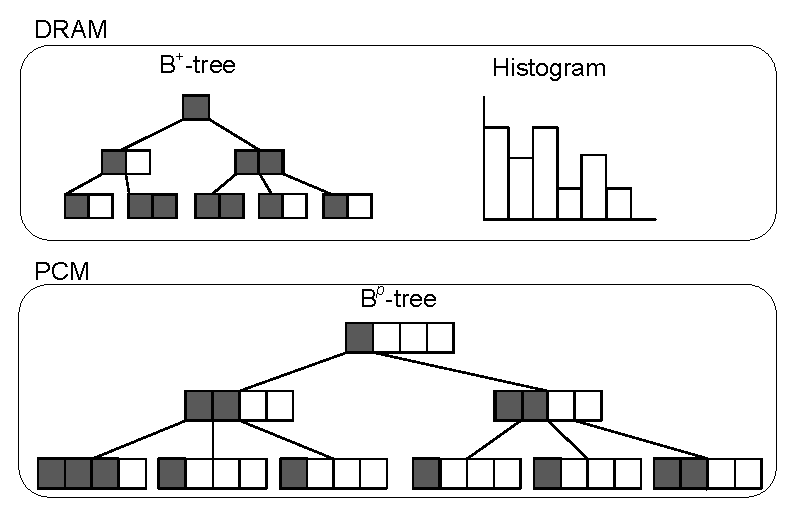
\includegraphics[scale=0.75]{figs/archi.eps}
\caption{\bptree architecture}
\label{fig:archi}
\end{figure}





%For simplicity, we assume \bptree a unique index, that is, there is exactly one record for each key value.
%\bptree is different, such that
%Details of the merge algorithm will be given in Section \ref{sec:algorithm}.
%Since our main idea relies on the prediction, we describe the detail of the prediction model in Section~\ref{sec:prediction}. After that, we describe the basic algorithms of the \bptree.
%\reminder{Add a figure of the architecture} A \bplustree in \pcm, a \bplustree in DRAM, a prediction model



\section{Main Components of {\large \bptree}}
\label{sec:algorithm}

In this section,
we will describe the details of the construction process
of a \bptree.
It consists of two phases, namely the warm-up phase and update phase,
which will be described in Section \ref{sec:warmup}
and Section \ref{sec:build} respectively.


For ease of presentation,
we summarize the notations used throughout this paper in Table~\ref{tab:notations}.

\begin{table}[!t]
\centering \caption{Notations}
\begin{tabular}{|l|p{6.5cm}|} \hline
Parameter&Description \\ \hline \hline
$h$&Height of the \bptree and \bplustree \\ \hline
$2M$&The branching factor of the \bptree on \pcm \\ \hline
$2m$&The branching factor of the \bplustree on DRAM \\ \hline
%$N$&Total number of entries of \bplustree \\ \hline
%$T$&Total number of entries of \bptree \\ \hline
$K$ & $M$ divided by $m$ ($K$ is an integer and $K \ge 1$)\\ \hline
%$b$ & The number of keys in a \bptree node \\ \hline
%$L_i$&Level $i(0\leq i \leq h$) of the tree \\ \hline
%$T_i$&Splitting threshold value of level i($0\leq i \leq h$) \\ \hline
%count$_L$&Number of entries localized in the extent of node L according to the \predict model \\ \hline
%frac$_L$&count$_L$ divided by N   \\ \hline
%$num_{bucket}$&Number of buckets in the histogram \\ \hline$bucket_i$($0$$\leq$$ i $$\leq$$ num_{bucket}$)
$B_i$ & The $i$-th bucket \\ \hline
$n_i$&Number of entries in the $i$-th bucket \\ \hline
\end{tabular}
\label{tab:notations}
\end{table}


\subsection{DRAM Buffer}

As new keys are inserted into the the DRAM buffer continuously,
a small standard \bplustree with branching factor
\emph{2m} is built in the DRAM buffer.
If the buffer is full,
we will flush the keys in the \bplustree to the \bptree on the \pcm.

To capture the data distribution,
we also maintain a histogram.
Suppose the range of the keys is $[L, U]$.
If we want to partition the keys into buckets $B_1, B_2, \cdots, B_{|B|}$,
the bucket width is $\frac{U-L}{|B|}$.
For each bucket $B_i$, we maintain the number of keys that fall in this bucket, denoted by $n_i$.
We will use the histogram to ``forecast'' the data distribution (Section~\ref{sec:model:warm}).

%%%%% lgl:start
%The DRAM buffer offers the following two advantages.
%Firstly, we can update the data in a batch manner onto the \pcm,
%%%% ooibc: check above
%%%% lgl: checked and modified
%which can reduce the number of writes.
%Secondly, we can get more accurate data distribution.
The main function of DRAM buffer is to adaptively adjust our predictive model based on the currently inserted keys in a time window. Then we can use the updated predictive model to merge all the keys in the time window in the \bplustree to the \bptree on \pcm.

%%%%% lgl:end



\subsection{Warm-up Phase} \label{sec:warmup}

Initially, the \bptree on \pcm is empty.
We use a DRAM buffer for warm-up.
We create a standard \bplustree for supporting insertions,
deletions and search.
Before the buffer is full, we use the conventional \bplustree for the initial operations.
For the first time that the DRAM buffer is full,
all the keys in the buffer will be moved to the \pcm,
and this step is called the warm-up process.
The main function of the warm-up phase is to
construct the skeleton of the \bptree on \pcm.

Suppose the DRAM buffer can accommodate $N$ keys.
We first predict the total number of possible keys.
Then, for each \bplustree node,
we use our \predict model to decide whether to split it
in an eager manner to avoid writes for subsequent insertions.
We will provide the details for constructing the initial \bptree
in Section~\ref{sec:model:warm}.


\begin{figure}[!t]
\centering
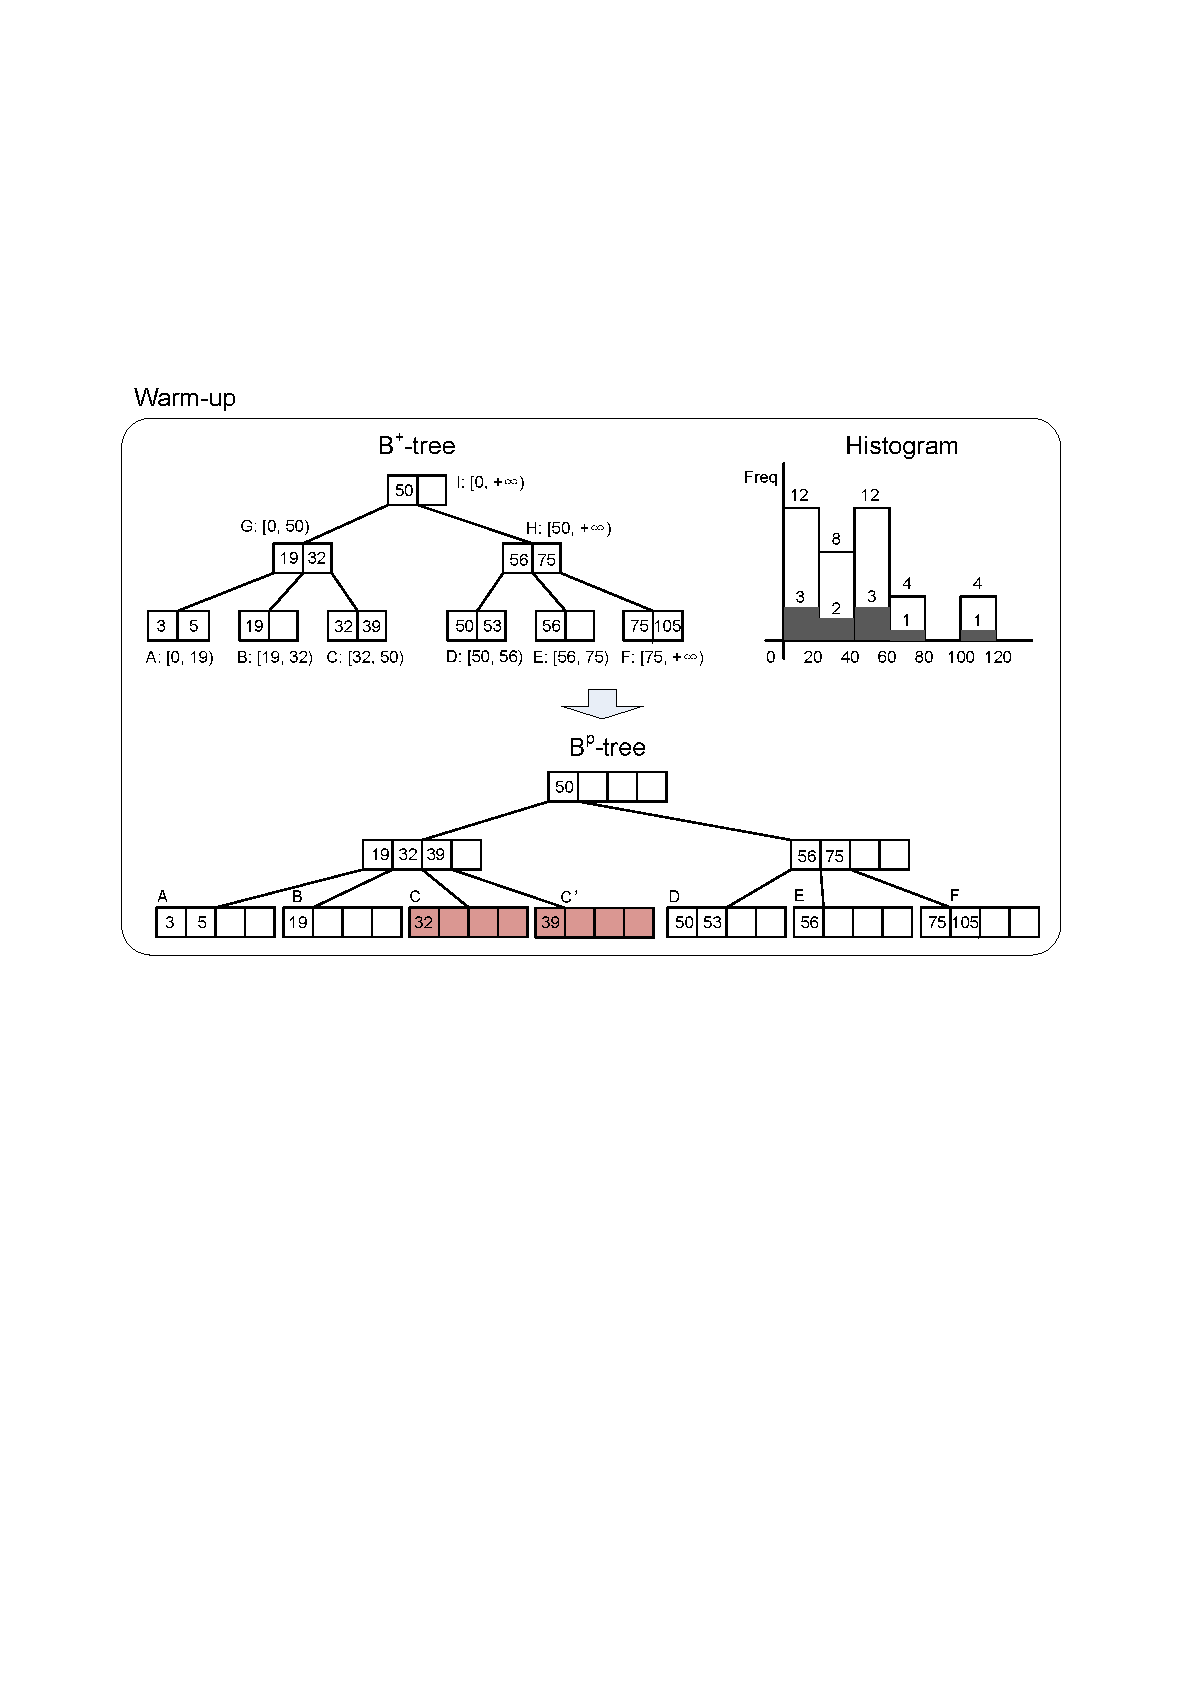
\includegraphics[scale=0.85]{figs/warmup.eps}
\caption{An example of a warm-up phase}
\label{fig:ex:warmup}
\end{figure}

Figure~\ref{fig:ex:warmup} shows an
example for the warm-up phase.
The \bplustree and histogram are in the DRAM and \bptree is in the \pcm.
In this example,
$N$ is 10 and the buffer is full and
thus we need to flush all the keys in the \bplustree to the \pcm.
The black portion of the histogram bar indicates the
number of inserted keys in each range so far, while
the whole bar indicates the predicted number of keys in each range
based on our \predict model.
From this figure,
we can observe that the structure of the \bptree is similar
to that of the original \bplustree.
However, there are two key distinctions.
First, the node could be split in an early manner
if it meets the requirement of node splits.
Second, some of the nodes could \emph{underflow}
due to either an enlargement of the node size or an early split.
These are guided by our \predict model and tree construction strategy.
In the example,
node $C$ in the B$^+$-tree is split into node $C$
and node $C'$ when it is moved to the \bptree,
nodes $B$ and $E$ underflow because of the enlargement of the node size,
while node $C$ and node $C'$ underflow because of the early split.
Details about the early split algorithm
will be presented in Section \ref{sec:model:warm}.

%and generate two nodes and  flush a key $k$ in \bplustree to
%The relative position of all keys in the tree will remain unchanged. We just need to enlarge the size of the tree node and copy all the keys and pointers in each node to the corresponding larger node on \pcm. At this time, the tree on the \pcm is quite sparse and empty, which we call stand of the \bptree.
%Here, \emph{M} is \emph{K} times greater than \emph{m}, that is, . \emph{K} is a parameter of \bptree and needs to be determined in advance.
% In \cite{hankins2003effect}, it has been proved that B$^+$-Tree with node size

%until the buffer is full. firstly insert into the buffer and build a small normal \bplustree. This is because we use it to facilitate the search query. We also need to update the histogram. When the buffer is full, the new \bplustree will be merged into the main \bptree on \pcm. We call each time the merge happens a \emph{time window}.




\subsection{Update Phase}\label{sec:build}

After the warm-up phase,
we have a \bptree structure on the \pcm.
Then for new operations,
we use both the DRAM buffer and
\bptree to handle the operations.
For an insertion, we insert it into the \bplustree.
%%%%% lgl:start
For a search query,
we search the key from both the \bplustree on DRAM and the \bptree on PCM.
If we find it, we return the answer; otherwise we return ``\emptyrst''. (Section~\ref{sec:model:update:search}).
%%%% ooibc: you need to search both regardless of what, as the DRAM buffered tree is a delayed insertion
%%%%  and there may already exist some similar keys in the bptree
%%%%  unless the keys are primary keys, but we do not make such assumptions here
For delete, we search it from both the \bplustree and the \bptree.
If we find it, we remove it from the \bplustree and the \bptree (Section~\ref{sec:model:update:deletion}).
%% TANKL: B+-tree don't need to remove key from non-leaf nodes!!
%The deletion operation on the \bptree has two differences from that on the standard \bplustree. First, we only remove the key from the leaf nodes and do not remove it from internal nodes. Second,
However, even if a node ``underflows'' after deletions, we do not merge it with its siblings. The reason is that since the read latency of PCM is much less
than the write latency, the overhead caused by empty nodes during
query processing is negligible. Furthermore, space could be reserved
for future insertion keys to reduce subsequent writes.
%%%% ooibc: same problem here
For update operation, like other indexes, we treat it as a deletion operation followed by an insertion.
The deletion operation does not need to be buffered, while the following insertion needs to be buffered first like the standard insertion operation on the \bptree.
%The reason we keep a small \bplustree in buffer is to facilitate the search query.
%%%% ooibc: this is not clear -- bigger buffer is better, but we do not have
%%%%       that much memory
Note that we need to update the histogram for the insertion and deletion operations.
If the DRAM buffer is full, we need to merge the \bplustree into the \bptree (Section~\ref{sec:model:update:insertion}).
%%%%% lgl:end


\begin{figure}[!t]
\centering
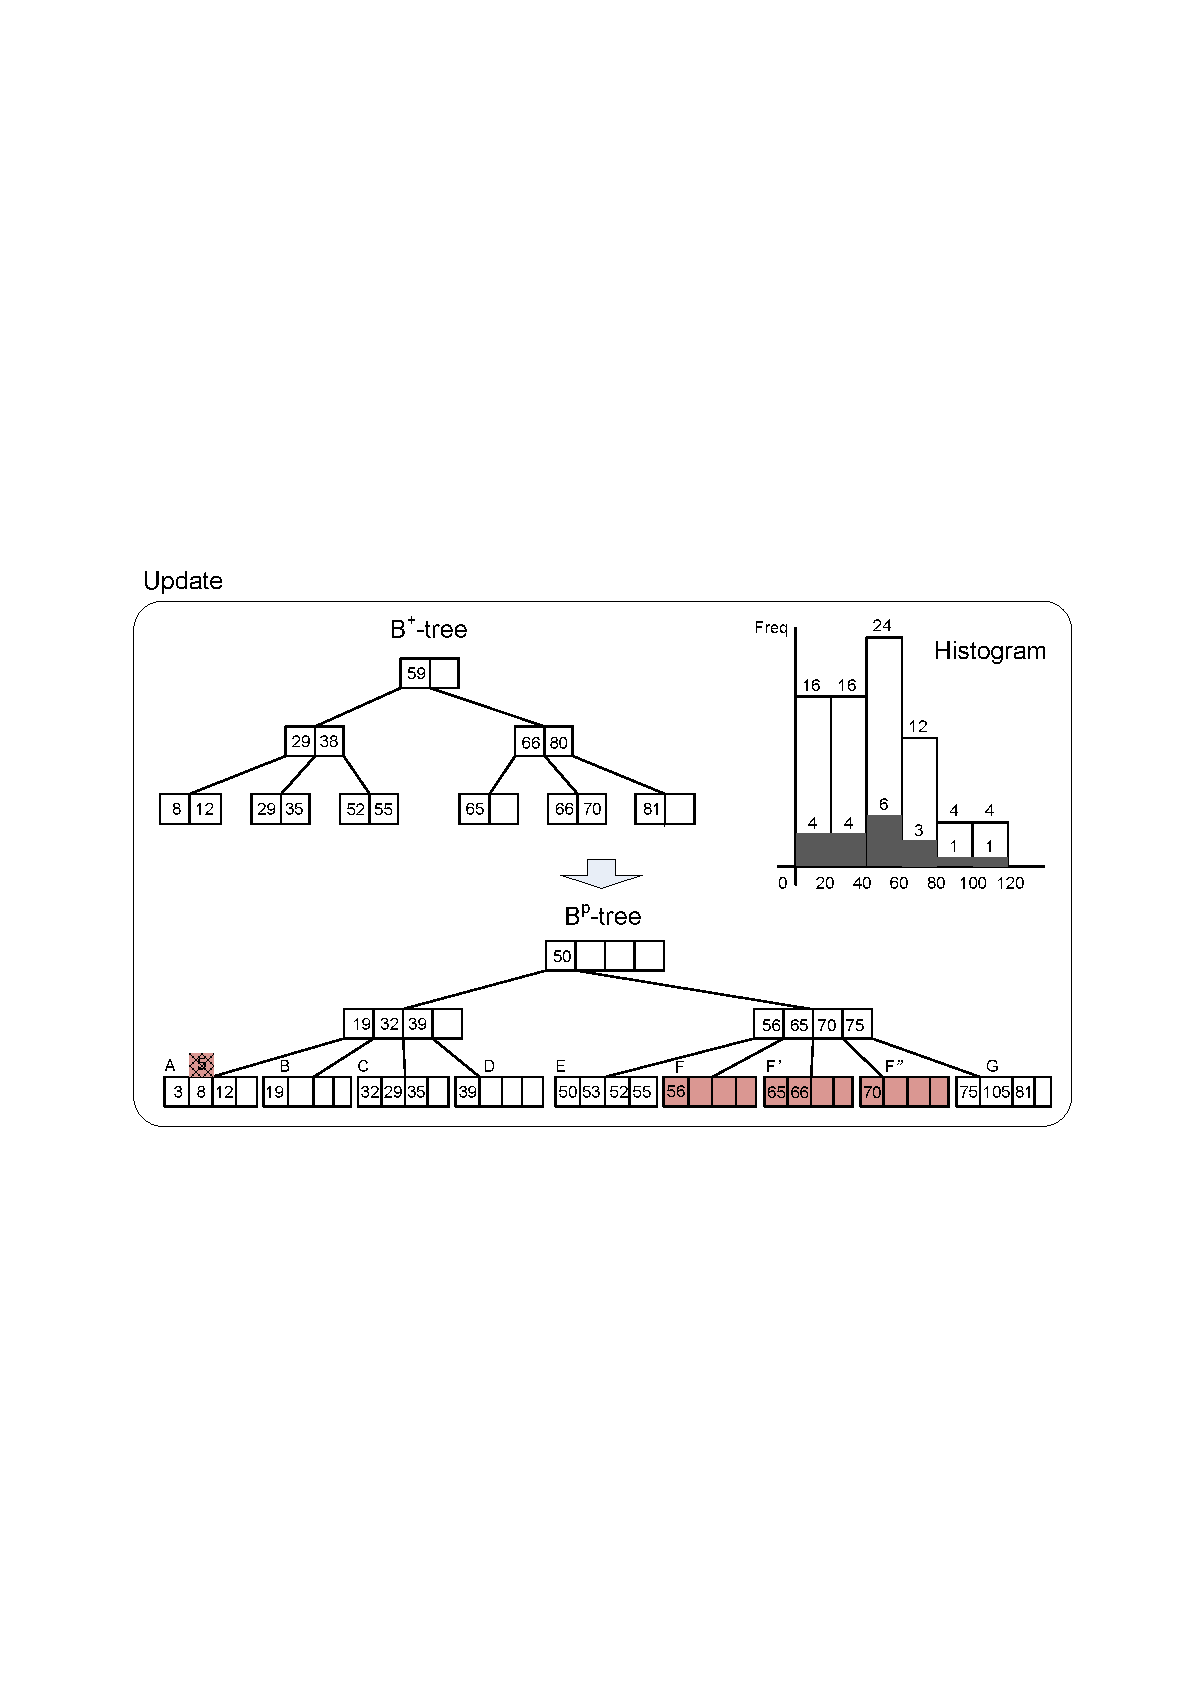
\includegraphics[scale=0.85]{figs/update.eps}
\caption{An example for update phase}
\label{fig:ex:update}
\end{figure}

Figure \ref{fig:ex:update} shows an example for update phase
affected on the earlier example described in Figure~\ref{fig:ex:warmup}.
The case in Figure~\ref{fig:ex:update} is that the buffer is
full for the second time and all the keys in the \bplustree are
merged into the \bptree described in Figure~\ref{fig:ex:warmup}.
In this example for the update phase,
we want to delete the key 5 in the \bptree index from Figure~\ref{fig:ex:warmup}.
First, we search the \bplustree in the buffer and cannot find it.
Then we search the \bptree on the
\pcm and find it in node $A$ and
subsequently remove it from the \bptree.
As can be seen from the figure,
the histogram is updated to reflect the effect of this deletion
and the new round of prediction is performed based on all the keys inserted
currently including the keys in the buffer.
Node $F$ in the \bptree is split because of the similar
reason as that of the node C in Figure~\ref{fig:ex:warmup}.
We will describe the details in Section~\ref{sec:model:update}.

\section{Summary}

In this chapter, we introduced our \bptree. We present the design principle and basic idea of \bptree. 
We know that there are two major parts of \bptree including the DRAM buffer and the normal \bplustree on \pcm. 
When new keys are inserted into the \bptree, there are two phases. First, the new key is inserted into 
the small \bplustree on the DRAM buffer, when the DRAM buffer is full for the first time, we merge the 
whole tree to \pcm and construct the skeleton of the tree on \pcm based on the predictive model. After 
that each time when the DRAM is full, we will merge the tree to the existing \bplustree on \pcm. 
During the construction, the node of our \bptree may be ``underflow'' which is different from the traditional
\bplustree. The reason is that sometimes we want to split the node in advance based on the prediction model even
the node is not full. In our design, even some nodes may be ``underflow'', we will still use some strategy to 
ensure that the whole tree is in a good shape. We will talk about the details about the prediction model 
and the construction process in next chapter. 

\newpage

\chapter{Predictive Model}
\label{sec:model}

In this chapter, we are going to present the predictive model which is a key part of our design. 
In the previous chapter, we have known that there are two major phases in our \bptree, both of
which will be based on this predictive model. Thus in this chapter, we will talk about how we 
construct the predictive model and use it in these two phases. We also know that the accuracy of 
the model is critical to the performance of the whole indexing and thus we will present our strategy 
to evaluate the realtime status of the predictive model and make adjustment to make it work properly. 
There will be three major parts of this chapter including the predictive model for warm-up phase, 
predictive model for update phase and evaluating \bptree. 

\section{Predictive Model for Warm-up} \label{sec:model:warm}


In this section, we introduce a \predict model to construct a \bptree structure in the warm-up phase. We will present running examples to show what the predictive model is and how it is integrated into our \bptree. We first discuss how to predict a \bptree skeleton (Section~\ref{subsec:model:warm:skeleton}), and then propose to construct a \bptree (Section~\ref{subsec:model:warm:insertion}).

\subsection{Predicting the {\large \bptree} Skeleton} \label{subsec:model:warm:skeleton}



Suppose there are $N$ keys in the DRAM \bplustree, the height of the \bplustree is $h$, and the branching factor is $2m$. The \bptree has the same height as the \bplustree, but with a larger branching order $2M=K*2m$, where $K$ is an integer and $K \ge 1$. $K$ can be set by the administrator. We can also predict $K$ as follows.

Let $T$ denote the total number of possible keys in the whole dataset. We  estimate $T$ using the numbers of keys in the histogram. Suppose the maximal number of keys in a bucket is $A$ and the bucket width is $W=\frac{U-L}{|B|}$, thus there are at most $W$ keys in a bucket. We use $N\times \frac{W}{A}$ to predict the possible key number $T$. As there are $T$ keys in \bptree and $N$ keys in \bplustree, we set $K=\log_h \frac{T}{N}$.

Obviously, if we overestimate $K$, the \bptree will turn out
to be sparse; on the contrary, if we underestimate the number,
we may need to do more splits.  We assume that each tree node
in the final \bptree is expected to be $\mu$\% full, i.e.,
each leaf node has $E=\mu\% \times 2M$ keys.
Thus the $i$-th level is expected to have $E^i$ nodes (the root is the first level, which has only one node).

After we got the number $K$, we can build the skeleton of the \bptree, in other words, we are going to enlarge the size of each node in the tree by $K$, 
in which case, there may be many ``underflow'' nodes. But we will not worry about this and we will gradually insert keys into these nodes and raise the average
node utilization. 

%the branching factor of the \bptree is set to $M=K*m$, where
%have three possible ways to get the number $T$. First, the number can be set by an administrator. Second, we suppose that all the numbers in the range $[L,U]$ will be inserted and thus $T=U-L$. Third, we

\subsection{{\large \bptree} Construction} \label{subsec:model:warm:insertion}




In this section, we discuss how to construct the \bptree based on the current \bplustree structure. We traverse the \bplustree in post-order. For each node, we predict whether we need to split it based on our \predict model (which will be introduced later). If we need to split it, we split it
into two (or more) nodes, and insert separators (or keys)
into its parent node, which may in turn cause the parent node to be split.
Following this approach, the process will continue to spread to the whole tree. 
As we employ a post-order traversal, we can guarantee
that the child splits are before the parent split,
and our method can keep a balanced tree structure.

Next we discuss how to split a \bplustree node. For ease of presentation, we first introduce a concept.

\begin{definition}[Node Extent] \label{def:extent}
Each node $n$ in the index tree is associated with a key range $[n_l, n_u]$, where $n_l$ and $n_u$ are respectively the minimum key and the maximum key that could fall in this node. We call this range the \textit{extent} of the node.
\end{definition}

The extent of node \emph{A} and \emph{B} of the \bplustree in Figure \ref{fig:ex:warmup}, for example, are $[0,19)$ and $[19,32)$ respectively. If a node is not the leftmost or the rightmost child of its parent, we can get its extent from its parent (except for the root node); otherwise we need to determine it from its ancestors. In practice, we need to update this information each time we split or merge nodes and we also need to consider this overhead in the evaluation. 


Consider a \bplustree node $n$ on the $i$-th level. Suppose its extent is $\elu$ and currently it has $|n|$ keys, \key{1}, \key{2}, $\cdots$, \key{|n|}. We access the keys in order. Suppose the current key is \key{j}. We next discuss whether to split the node according to \key{j} as follows. As $\el$ is the possible minimum key in the node, we first estimate the number of possible keys between $\el$ and \key{j}, denoted by $P(\el, \key{j})$. Then we estimate the number of keys that can be accommodated between \el and \key{j} on the \bptree, denoted by $A(\el, \key{j})$.


Obviously if $P(\el, \key{j})<A(\el, \key{j})$, we do not need to split the node according to \key{j}; otherwise we need to split the node. We generate a \bptree node with keys \el, $\cdots$, $\key{j-1}$, remove the keys \el, $\cdots$, $\key{j-1}$ from the DRAM \bplustree node, insert the key $\key{j}$ to its parent on DRAM \bplustree, and update the pointers of the \bplustree node: the left pointer of this key points to the \bptree node, and the right pointers of this key points to the \bplustree node. Next we repeatedly split the node with keys $\key{j}, \cdots, \key{|n|}$ (Note that \key{j} turns to the first key in the new node). If we cannot split the node for the last key, we will create a \bptree node with the same keys in the \bplustree node, and update the pointer of its parent to the \bptree node. Next we discuss how to predict $A(\el, \key{j})$ and $P(\el, \key{j})$.

\mbox{}

\subsubsection{Predicting the number of possible keys between \el and \key{j}:} 
If \el and \key{j} are in the same bucket $B_s$, we can estimate $P(\el, \key{j})$ as follows. Based on the histogram, there are $n_s$ keys in the bucket. Then the number of keys between \el and \key{j} can be estimated by (\key{j} - \el) $\times \frac{n_s}{W}$, where $W$ is the bucket width. Thus the number of possible keys in the range is

\begin{equation}
P(\el, \key{j}) = K \times  (\key{j} - \el) \times \frac{n_s}{W},
\end{equation}

\noindent if \el and \key{j} are in the same bucket $B_s$.

On the contrary, if \el and \key{j} are in different buckets, we estimate the number as follows. Without loss of generality, suppose \el is in bucket $B_s$ and \key{j} is in bucket $B_e$. Let $B_s^u$ denote the upper bound of keys in bucket $B_s$ and $B_e^l$ denote the lower bound of keys in bucket $B_e$. Thus the number of keys between \el and \key{j} in bucket $B_s$ is ($B_s^u$-\el) $\times \frac{n_s}{W}$. The number of keys between \el and \key{j} in bucket $B_e$ is (\key{j} - $B_e^l$) $\times \frac{n_b}{W}$. Thus the total number of keys between \el and \key{j} is ($B_s^u$-\el) $\times \frac{n_s}{W}$ + $\sum_{t=s+1}^{e-1} n_t$ + (\key{j} - $B_e^l$) $\times \frac{n_b}{W}$. Thus the number of possible keys between \el and \key{j} is
\begin{equation}\hspace*{-2em}P(\el, \key{j}) = K \times \bigl( (B_s^u-\el) \times \frac{n_s}{W} + \sum_{t=s+1}^{e-1} n_t + (\key{j} - B_e^l) \times \frac{n_b}{W} \bigr),
\end{equation}
\noindent if \el and \key{j} are in different buckets.


\mbox{}

\subsubsection{Predicting the number of keys that can be accommodated between \el and \key{j}:} 

Note that node $n$ has $|n|$ keys and it is expected to have $E$ keys, thus the number of accommodated keys in this node is $E-|n|$. Thus $$A(\el, \key{j}) = \min(\key{j}-\el, E-|n|),$$ if $n$ is a leaf node.

If node $n$ is a non-leaf node, we can directly add $j$ children between the two keys. In addition, we can also add some keys between \el and \key{j} as there are $E-|n|$ positions which are not used in the node. Obviously, we insert
at most $\min(\key{j}-\el, E-|n|)$ keys in the node. Thus we can add at most
$c=j+\min(\key{j}-\el, E-|n|)$ children under the node between \el and \key{j}. As node $n$ is in the $i$-level, the children are on $i+1$-level. As each child can have $E$ keys and $E+1$ children, each node can have $(E+1)^{h-i-1}$ descendants. Thus there are $c\times \sum_{t=0}^{h-i-1}(E+1)^t$ nodes between the two keys. As each node can accommodate $E$ keys, the total number of accommodated keys is
\begin{equation}
A(\el, \key{j})=E\times c\times \sum_{t=0}^{h-i-1}(E+1)^t,
\end{equation}
\noindent if node $n$ is a non-leaf node.


\begin{figure}
\linesnumbered \SetVline \setcounter{algocf}{0}
\begin{algorithm} [H]
\KwIn{\bplustree and Histogram in DRAM Buffer}
\KwOut{\bptree on PCM}
%\label{alg:warmup}
\Begin{
    Let $r$ denote the root of the \bplustree, Level $i=0$ \;
    \postorder($r$, $i$, Histogram) \; \nllabel{alg:warmup:postorder}
}
\caption{Warm-up(\bplustree, Histogram)}
\end{algorithm}

\begin{function}[H]
\KwIn{$n$: \bplustree node; $i$: Level of $n$; Histogram}
 \KwOut{\bptree nodes}
  \Begin{
        \For{each child $c$ of $n$}
        {
            \postorder($c$, $i+1$, Histogram)\;
        }
        \key{j} = \splitfunc($n$, $i$, Histogram)\; \nllabel{func:postorder:split}
        \While{$\key{j}~!=~\phi$}
        {
            Generate a \bptree node with \el,$\cdots$,\key{j-1}\; \nllabel{func:posorder:generatesplit}%branching order $M$ and
            Remove keys after $\key{j}$ from \bplustree node $n$\; \nllabel{func:posorder:remove}
            Insert \key{j} to the parent of $n$ on \bplustree and update the pointers \; \nllabel{func:posorder:insert}
            %: the left pointer of this key to the \bptree node, and the right pointers of this node to the \bptree node\;
            Split($n$, $i$, Histogram)\; \nllabel{func:posorder:split2}
        }
        Create a node with \el,$\cdots$,\key{j-1}, remove $n$, update $n$'s parent\;
        \nllabel{func:posorder:generatesnonplit}
        % of node $n$ to this \bptree node \; %branching order $M$ and keys
 }
        \caption{\postorder($n$, $i$, Histogram)}
\end{function}
\begin{function}[H]
\KwIn{$n$: \bplustree node; $i$: Level of $n$; Histogram}
 \KwOut{Key: Split Key}
  \Begin{
        Let \el denote the first key in node $n$ \;
        \For{$j=2, 3, \cdots |n|$}
        {
            \If{\predictkeys(\el, \key{j}, $i$)}
            {
               return \key{j} ;
            }
        }
        return $\phi$ \;
        \caption{\splitfunc($n$, $i$, Histogram)}
 }
\end{function}
\begin{function} [H]
\KwIn{\el; \key{j}; Histogram}
 \KwOut{True or false}
  \Begin{
        Compute A(\el, \key{j}); %the number of keys between \el and \key{j} that can be accommodated in \bptree\;
        Compute P(\el, \key{j}) \; %the estimated number of keys between \el and \key{j} \;
        \lIf{$A(\el, \key{j})<P(\el, \key{j})$}
        {
            return true;
        }

        \lElse
        {
            return false;
        }
        \caption{\predictkeys(\el, \key{j}, Histogram)}
 }
\end{function}
        \caption{Warmup Algorithm} \label{alg:warmup}
         \setcounter{algocf}{1}
\end{figure}


To summarize, we can use the predicted numbers to split the nodes. Iteratively, we can split all the nodes and insert the new nodes into PCM. Figure~\ref{alg:warmup} illustrates the algorithm. The \warmup algorithm first traverses
the \bplustree in post-order by calling its function \postorder (line~\ref{alg:warmup:postorder}). Function \postorder splits the nodes iteratively. Given a node $n$ on level $i$, it checks
whether the node should be split by calling function \splitfunc (line~\ref{func:postorder:split}), which is used to split a node based on our \predict model. If our model decides to split node $n$, we generate a \bptree node with keys, \el, $\cdots$, $\key{j-1}$ (line~\ref{func:posorder:generatesplit}), remove the keys, \el, $\cdots$, $\key{j-1}$, from the DRAM \bplustree node (line~\ref{func:posorder:remove}), insert the key $\key{j}$ to its parent on DRAM \bplustree (line~\ref{func:posorder:insert}), and update the pointers of the \bplustree node: the left pointer of this key to the \bptree node, and the right pointers of this key to the \bplustree node. Next we repeatedly split the node with keys, $\key{j}, \cdots, \key{|n|}$ (line~\ref{func:posorder:split2}). If we cannot split the node for the last key, we will create a \bptree node with the keys, and update the pointer of its parent to the \bptree node (line~\ref{func:posorder:generatesnonplit}). Iteratively, we can construct the \bptree structure.

We show an example of the split algorithms in Figure~\ref{fig:ex:warmup}. Here we take the leaf node for an example instead of the whole split algorithm. As can be seen from the Figure~\ref{fig:ex:warmup}, the previous node $C$ is split into two nodes $C$ and $C'$, though it is not full. Since there are only two keys in previous node $C$, we shall calculate A(\el, \key{2}) and P(\el, \key{2}) as follows. A(\el, \key{2}) $= \min(39 - 32, 4 - 2) = 2$, P(\el, \key{2}) $= (39 - 32) * \frac{8}{20} = 2.8$. As A(\el, \key{2}) $<$ P(\el, \key{2}), according to the algorithms in Figure \ref{alg:warmup}, node $C$ needs to be split and a new node $C'$ is created and then we update the pointers.

\section{Predictive Model for Updates}  \label{sec:model:update}


In this section we propose a \predict model for the update phase. We will describe the basic operations on a \bptree, including search (Section~\ref{sec:model:update:search}), deletion (Section~\ref{sec:model:update:deletion}), and insertion (Section~\ref{sec:model:update:insertion}). Actually the search and deletion processes are similar to that of the standard \bplustree (except the need
to deal with unordered leaf entries). Thus
our main focus will be on the insertion.

\subsection{Search}\label{sec:model:update:search}

Since we use a small DRAM as a buffer, some
newly inserted keys will still be in the main memory \bplustree and
have not been merged into the main \bptree on PCM.
%Thus, both the \bplustree and \bptree need to be searched.
Thus, besides searching the main \bptree in the manner similar to that of the \bplustree, for our \bptree, a search operation still needs to search the small \bplustree first. Then there will be two steps in the search process.
We first lookup the small \bplustree in the buffer, and then search the main \bptree. As noted, since the entries within a leaf node of the \bptree may not
be sorted, the search will examine every key entry.
If neither of the two steps return any results, \textsf{null} will be returned. The above steps are summarized in Figure~\ref{alg:search}.
Obviously the time complexity of the search operation is $\mathcal{O}(h)$, where $h$ is the height of the \bptree and it is similar to the traditional \bplustree.


\begin{figure}[!t]
\linesnumbered \SetVline \setcounter{algocf}{1}
\begin{algorithm}[H]
\caption{Search(\bplustree, \bptree, \key{})}
\KwIn{\bplustree; \bptree; A search \key{}}
\KwOut{Search result}
\label{alg:alg3}
\Begin{
    Search both the \bplustree and \bptree using \key{} \;
    \If{Find \key{} in \bplustree or find \key{} in \bptree}{
        return the entry or entries;
    }
    \Else {
        return \textsf{null}\;
    }
}
\end{algorithm}
\caption{\bptree: Search Operation}\label{alg:search}
\end{figure}

\subsection{Deletion}\label{sec:model:update:deletion}

Like search, deletion also requires searching both \bptree and \bplustree.
A deletion on the \bptree is handled in a similar way as that for
standard \bplustree, but with some differences.
%The first difference is that we only remove the key in the leaf nodes and do not remove it from internal nodes. The second one is that
First, the deleted entry can be replaced by the last key entry in the
node. This is to pack the entries within the leaf node.
Second,
if the corresponding leaf node has fewer than $M$ keys, we will not borrow keys from its siblings. This can avoid the merge operations. The reason is that since the read latency of PCM is much shorter than the
write latency, the overhead caused by the empty node in the query processing stage is negligible. Furthermore, the space could be reserved for the future keys to reduce subsequent writes.



Given a key to delete, we first search it from the \bplustree. If we find the entry, we directly remove it from \bplustree. If not, we then search it in the \bptree. If we find the leaf node in the \bptree, we remove the key from the node. Note that we will not do merge operations even if the node has less than half (M) keys. We do not propagate the deletion operation to its ancestors. The above steps are summarized in Figure~\ref{alg:deletion}. Obviously the time complexity of the deletion operation is $\mathcal{O}(h)$.



\begin{figure}[htup]
\linesnumbered
\begin{algorithm}[H]
\caption{Delete(\bplustree, \bptree, \key{})}
\KwIn{\bplustree, \bptree, \key{}}
\KwOut{Delete status}
\label{alg:alg2}
\Begin{
    result $\leftarrow$ false \;
    Search the \bplustree using \key{} \;
    \If{Find \key{} in \bplustree}{
        delete the entry in a \bplustree operation manner\;
        result $\leftarrow$ true \;
    }
    Search the \bptree using \key{} \;
    \If{Find \key{} in \bptree}{
        remove the entry from the leaf node\;
        result $\leftarrow$ true \;
    }
    return result \;
}
\end{algorithm}


\caption{\bptree: Deletion Operation}\label{alg:deletion}
\end{figure}


\subsection{Insertion}\label{sec:model:update:insertion}

Since \bptree is maintained with the aid of a DRAM buffer and a \predict model, both the \bplustree in the buffer and the histogram of the \predict model need to be updated in each insertion. When the buffer is full, the \bplustree will be merged into the main \bptree on PCM.


All the keys in the \bplustree will be inserted into the main tree one by one. Once a key is to be inserted, we first look up the leaf node \emph{L} that the new key belongs to as the standard \bplustree. Then we predict whether it should be directly inserted into the node or the node should be split. We first compute the number of keys that can be accommodated in this node $L$, denoted by $ANO_L$. We then predict the number of keys that could fall in this node, denoted by $PNO_L$. If $PNO_L\geq ANO_L$, we need to split the node; otherwise, we will not. If we need to split the node, a new leaf node will be created and a ``middle'' key will be chosen based on the \predict model and pushed upward to the parent node. Existing keys in the node \emph{L} needs to be adjusted according to the ``middle'' key.


Note that the middle key is not the key in the median position as the standard \bplustree. Instead, we need to select a median key based on the data distribution (which will be discussed later). As we insert a middle key into its
parent, it may cause its parent to split. The above steps are summarized in Figure~\ref{alg:insertion}.  Next, we discuss how to compute $PNO_n$ and $ANO_n$ for node $n$.

\mbox{}

\subsubsection{Computing the accommodated key number of node $n$, $ANO_n$:} 

Suppose node $n$ is in the $i$-th level. Each node has at most $2M$ keys and 2M+1 pointers, thus node $n$ has $\sum_{t=1}^{h-i} (2M+1)^{t}$ descendants. Thus the accommodated key number of node $n$ is
\begin{equation}ANO_n=2M*\sum_{t=0}^{h-i}(2M+1)^t.\end{equation}


%its parent based on the pointer and finds the lower bound of keys in this node \el and the lower bound of keys in this node \eu.

\mbox{}

\subsubsection{Predicting the possible key number occupancy in node $n$, $PNO_n$:} 

Next we predict the total number of keys that could potentially belong to this node. We first find the extent of this node, denoted by $\elu$, where $\el$ and $\eu$ are respectively the minimum key and the maximum key in this node. Based on the two bounds, we can compute the number of possible keys fell into this node as discussed in Section~\ref{subsec:model:warm:insertion}.

That is if \eu and \el are in the same bucket $B_s$,

\begin{equation}PNO_n = K \times  (\eu - \el) \times \frac{n_s}{W};\end{equation}


\noindent otherwise if \el and \eu are respectively in two different buckets $B_s$ and $B_e$.

\begin{equation}PNO_n = K \times \bigl( (B_s^u-\el) \times \frac{n_s}{W} + \sum_{t=s+1}^{e-1} n_t + (\eu - B_e^l) \times \frac{n_b}{W} \bigr).\end{equation}


Based on $ANO_n$ and $PNO_n$, we can decide whether to split a node $n$. Next we discuss how to select a middle key if we need to split a node.


\mbox{}

\subsubsection{Computing the middle key in node $n$, $midKey$:}
Consider the keys in $n$ are \key{1}, \key{2}, $\cdots$, \key{|n|}. Without loss of generality, suppose \key{1} $\leq$ \key{2} $\leq$  $\cdots$ $\leq$ \key{|n|}. Based on extent of a node, we define the middle key formally.



\begin{definition}[Middle Key]
A key $\key{i}$ in node $n$ is called a middle key if $$P(\el, \key{i})\leq \frac{P(\el, \eu)}{2},$$ $$P(\el, \key{i+1})>\frac{P(\el, \eu)}{2},$$ where $P(\key{i}, \key{j})$ denote the number of predicted keys between \key{i} and \key{j}.
\end{definition}

A straightforward method to find the middle key from a node is to compute $P(\el, \key{i})$ for each $i$ from $1$ to $|n|$ until we find the middle key. The complexity is $\mathcal{O}(M)$. If the keys are sorted, e.g., the keys in an internode, we can use an alternative method. We have an observation that if the keys are sorted, $P(\el, \key{i})\leq P(\el, \key{j})$ for $i<j$ as formalized in Lemma~\ref{lemma:seq}. Thus we can employ a binary search method to find the middle key and reduce the time complexity to $\mathcal{O}(\log M)$. If the keys are unsorted, the complexity is $\mathcal{O}(M)$.


\begin{lemma} \label{lemma:seq}
Given a node $n$ with keys ordered as
\key{1}, \key{2}, $\cdots$, $\key{|n|}$, and two keys $\el\leq \key{1}$ and $\eu\geq \key{|n|}$, we have $$P(\el, \key{i})\leq P(\el, \key{j})$$ for $i<j$.
\end{lemma}


Thus the worst-case time complexity of an insertion operation is $\mathcal{O}(M+h \times \log M)$, where $M$ is the branching factor and $h$ is the height.




\begin{figure}[!t]
\linesnumbered
\begin{algorithm}[H]
\caption{Insert(\bplustree, \bptree, \key{})}
\KwIn{\bplustree, \bptree, \key{}}
\KwOut{Updated \bptree}
\label{alg:alg1}
\Begin{
    Search the leaf node for \key{}, $L$ \;

    \upgrade(L, Histogram)\;
}

\end{algorithm}


\begin{function} [H]
\KwIn{$n$: A \bptree node, Histogram}
  \Begin{
       $PNO_n \leftarrow $ GetPredictedNumber($n$)\;
        $ANO_n \leftarrow $ GetAccomodatedNumber($n$)\;
        \If{$PNO_n < ANO_n$}{
            insert \key{} into $n$\;
            return\;
        }
        \Else{
            $midKey \leftarrow GetMiddleKey(n)$\;
            $midKey$ is pushed upward to the parent $p$ \;
            A new leaf node $n'$ is created and new pointer from the parent node to $n'$ \;
            Remove keys larger than $midKey$ from $n$ to $n'$ \;
            \upgrade($p$, Histogram) \;
        }
        \caption{\upgrade(n, Histogram)}
 }
\end{function}

\caption{\bptree: Insertion Operation}\label{alg:insertion}
\end{figure}

\section{Evaluating {\large \bptree}}
\label{sec:cost}

In this section, we introduce several metrics to evaluate
the status of \bptree and use them to guide the future prediction which is necessary to keep the tree balanced.

The first metric is insertion overflow.
When inserting a new entry into the \bptree, we employ a leaf-to-root way, that is we always insert a key into leaf node first. If the node overflows, it needs to be split and some of the keys need to be moved to other nodes.
%% TANKL: our bptree adopts "unsorted leaf" strategy now. so the following
%%        paragraph is no longer valid
%When we insert a key into the leaf node, we need to insert it into a specific position to guarantee the order of keys. In this case, we need to move the keys larger than the inserted key. Moreover if the parent needs to split, we need to repeat the operations. Although we can make the keys unordered~\cite{chen2011rethinking}, it may decrease the performance, especially for internal nodes.
Obviously, the larger the number of keys in a node is, the higher is the
probability for it to split and the overhead incurred
to move keys. Thus we can use the number of keys in a node to
evaluate the degree of insertion overflow.
Given a node $n$ with $n_{keys}$ keys.
A larger $n_{keys}$ implies there is a higher probability for $n$
to split, resulting in a larger number of possible writes.

%Let $n_{w}$ denote the number of writes and $n_{in}$ denote the number of insertions. If $n_{w}>\delta n_{in}$, for example $\delta=\frac{h}{3}$, we need to lots of writes, and we need to rebuild the \bptree.


The second metric is unqualified-node ratio. A node is called an \emph{unqualified node} if its key number is smaller than $M$. If there are many unqualified nodes, the constructed \bptree is very sparse. For a node $n$, the
smaller the value of $n_{keys}$, the sparser the tree will be.
To evaluate the overall \bptree, we need to consider all tree nodes. Let $n_{un}$ denote the number of unqualified nodes.
The larger the value of $n_{un}$,
the sparser the \bptree. We can easily determine $n_{un}$
as follows. Initially, all nodes are unqualified nodes and $n_{un}$ is the total number of nodes. When inserting a key, if an unqualified node turns to be a qualified node (with key number no smaller than $M$), we decrease the number $n_{un}$ by 1.

Next we combine the above two factors to evaluate a \bptree. As the expected utilization is $\mu\%$ and then the average key number of a node is $\mu\% \times 2M$, we can use the following equation to evaluate the \bptree,

\begin{equation}Q=\sum_n \delta \times (n_{keys}- \mu\% \times 2M),\end{equation}

\noindent where

\begin{equation}
  \delta = \left\{
   \begin{array}{ll}
   \frac{n_{keys}}{\eu-\el}  & n_{keys}\geq \mu\% \times 2M \\
   \\
   \frac{\eu-\el}{n_{keys}} &  n_{keys}< \mu\% \times 2M \\
   \end{array}
  \right.
\end{equation}
\noindent and $\elu$ is the extent of node $n$, in \cite{DBLP:journals/csur/Comer79} $\mu$ is 69 for the standard \bplustree .

\mbox{}

If $Q$ is larger than 0, then it means that the
\bptree is very dense. The larger the value of $Q$, the denser the \bptree
will be. However it may involve many more numbers of writes when the
tree needs to be reorganized (by splits and merges).
If $Q$ is larger than an upper bound $\tau_u$, we need to tune our model
to do more (planned) splits (when merging \bplustree with \bptree).

On the contrary, if $Q$ is smaller than 0, \bptree is very sparse.
The smaller the value of $Q$, the sparser the \bptree. If $Q$ is smaller
than a lower bound $\tau_l$, we need to tune our method to reduce
the number of (planned) splits.


%Thus we can tune the tree structure based on this metric.
%If $n_{un}$ is in $[M, 2M]$, the \bptree is very robust. If $n_{un}<\tau$, for example $\tau=M/2$, we need to rebuild the \bptree.
%The number of writes of inserting a node to the leaf is $(M+2)\times n_{io}$.
%If we the corresponding leaf node is not overflow, we directly insert to the leaf node; otherwise we insert the median of the node into its parent, allocate a new leaf node, and move the half the node's elements into the new node. We need to copy $M$ data into the new node and insert the median to the parent and add the two children links to the two nodes\reminder{add the number of writes inserting a data into the leaf and intermedin nodes}. The number of writes is $(M+2)$. Let $n_{io}$ denote the number of asbestoses of the node that needs to be split. The number of writes of inserting a node to the leaf is $(M+2)\times n_{io}$.




\iffalse
$PNO_L \leftarrow $ GetPredictedNumber($L$)\;
    $ANO_L \leftarrow $ GetAccomodatedNumber($L$)\;
    \If{$PNO_L \leq ANO_L$}{
        insert \key{} into $L$\;
        return\;
    }
    \Else{
        $midKey \leftarrow GetMiddleKey(L)$\;
        $midKey$ is pushed upward to the parent $p$ \;
        A new leaf node $L'$ is created and new pointer from the parent node to $L'$ \;
        Remove keys larger than $midKey$ from $L$ to $L'$ \;
        \upgrade($p$, Histogram) \;
    }
\fi
%Note that we can keep the value $n_{io}$ for each node

\section{Summary}
In this chapter, we introduced the predictive model we use to construct the \bptree. There are two phases when constructing the tree including 
the warm-up phase and the update phase. The warm-up phase means the time before the first time that the DRAM buffer is full and after that we 
start the update phase. In both phases, the predictive model is very important and it will influence whether we will split a node in advance or not. 
Then we talked about the normal operations of our \bptree and we gave the detailed algorithms. After that we proposed a evaluating model to evaluate the 
realtime status of our predictive model and some metrics are adopted to make it work properly and further ensure a good status of the whole indexing tree. 

\newpage

\chapter{Experimental Evaluation}
\label{sec:experiment}


In this chapter, we evaluate the performance of our proposed
\bptree and show the experimental results. An extensive performance study is conducted to show the
efficiency and effectiveness of the \bptree with various types of
queries and updates. Since we have not got any PCM prototype in hand, we need to setup an environment
to simulate the PCM characteristics first. Then we did our experiments in the simulated environment.
Our results show \bptree outperforms the traditional \bplustree on the insertion and deletion performance,
while holding a similar search performance at the same time.

\section{Experimental Setup}

In this section, we are going to present our experimental setup. We talk about the
experimental platform first and we will present the details of our simulation platform.
After that we will propose our data set, workloads and the different algorithms we are going to compare with.

\subsection{Experimental platform}

We integrate our proposed
\bptree in PostgreSQL and extend the buffer management module to
support the PCM model. We follow the specifications of the PCM
model in~\cite{chen2011rethinking} and we also talked about this in Chapter~\ref{sec:technology}.
Three metrics are used in our
experiments to measure the performance the \bptree, namely the
number of writes, energy consumption and CPU cycles.
%
Each time when we write a new cache line into the PCM, we compute the number
of modified bits and bytes by comparing it with the previous one.
In our experiments, the number of writes is computed as the
number of modified bytes, while the energy consumption is estimated
by the number of modified bits. We compute the CPU cost by
combining the CPU cycles of our \bptree in both PCM and DRAM.
%For the CPU cycles, we  the CPU cost of the \bplustree in DRAM buffer of our \bptree.

The experiments were conducted in CentOS release 5.6 with g++
4.1.2. Our system is powered with a 16-core Intel Xeon E5620
2.4GHz CPU and 64GB main memory. Based on the benchmark used
in~\cite{chen2011rethinking,qureshi2009scalable,bedeschi2008multi},
we set the parameters as follows: the read latency of a PCM cache
line is 288 cycles; the write latency of PCM is 281 cycles for
every 4 bytes; the read latency of a DRAM cache line is 115 cycles
and the write latency of DRAM is 7 cycles for every 4 bytes. In
PCM, the energy consumption is estimated as: the read energy per
bit is 2pJ and the write energy per bit is 16pJ. In
Table~\ref{tab:parameter}, we list the other parameters used in
our experiments and their value ranges.


\begin{table}\vspace*{-1em}
\centering
\caption{Parameters and their value ranges}
\label{tab:parameter}
\hspace*{-1em}
\begin{tabular}{|c|c|}
 \hline
 \bf Parameter & \bf Value Ranges \\
 \hline
 \hline Size of DRAM buffer&5\% of the size of the PCM used\\
 \hline Size of cache line&64B\\
 \hline Size of the \bplustree node& 256B (4 cache lines)\\
 \hline Size of the \bptree node&256B, 512B, 1024B \\
    &(4, 8, 16 cache lines)\\
 \hline K&1, 2, 4\\
 \hline Number of keys in &5 millions\\
    the data set & \\ \hline
\end{tabular}
\end{table}

%\vspace{.5em}

\subsection{Data sets and workloads}

Two synthetic datasets
are used in our experiments. One is generated to follow the
uniform distribution, while the other one follows the skewed
distribution. We generate 5 millions keys in each dataset. In our
experiments, the node size of the DRAM \bplustree is 256B, which
is equivalent to 4 cache lines; whereas the node size of all tree
structures on the PCM varies from 256B, 512B to 1024B. In our
\bptree, each index entry contains a 4-Byte key and a 4-Byte
pointer. The size of the DRAM buffer used is approximately 5\% of
the size of the PCM. We generate various workloads (i.e.,
insertions, updates and searches) to study the performance of our
approach. Specifically, an update is processed as a deletion
operation followed by an insertion operation, and the search
queries are composed of both the point queries and range queries.
Based on our experimental results, we find that the performance on
uniform dataset is similar to that on skewed dataset. Therefore,
we only report the results on skewed dataset.

\vspace{.5em}

\subsection{Algorithms compared}

We compare four different
indexing structures including our \bptree, the traditional
\bplustree, the proposed Unsorted Leaf tree
in~\cite{chen2011rethinking} and our \bptree with sorted leaf
nodes on the basis of the following measures, the number of writes during the insertions, the energy consumption,
the CPU cycles (including the small \bplustree in the DRAM for \bptree) during the insertions and searches, and the leaf nodes utilization.

As the \bptree is a composite structure including the main \bptree
on PCM and the small buffer \bplustree on DRAM, we need to
determine how to compute each performance metric first. In the
performance evaluation, we only consider the PCM cost while
calculating the number of writes and the energy consumption. As
for the CPU cost, the CPU cycles occupied for manipulating the
DRAM \bplustree are recorded, which can represent a more accurate
processing time. All the indexes are tuned and only the best results are reported.

In all figures presented in this section, ``BP-tree'' represents
our \bptree; ``B-tree'' represents the traditional \bplustree;
``Unsorted'' represents the proposed unsorted leaf tree
in~\cite{chen2011rethinking}; and ``BP-minus'' represents \bptree
with sorted leaf nodes. The x-axis represents the node size of the
corresponding tree, e.g., x-coordinates 4 indicates that the node
size of the corresponding tree is 4 cache lines.

\section{Results and Analysis}

We did various of experiments and in this chapter, we will show the results including insertion, update, search and node utilization.
At last, we also did some more experiments to show that our \bptree indexing can work well under different data distributions.

\subsection{Insertion}
We first evaluate the insertion performance of \bptree. We insert
all the keys in the dataset back-to-back using the different indexing algorithms. 
%and the measures include number of writes, energy consumption and CPU cycles.
Moreover, for each data set, we build the tree using three different node sizes, that is, 4, 8, 16 cache lines, respectively.

\begin{figure*}[!t]
\centering

\subfigure[Writes]{
    \includegraphics[scale = 0.55] {figs/zipf_result11.eps}
    \label{fig:exp:insertion:subfig12}
} \subfigure[Energy]{
    \includegraphics[scale = 0.55] {figs/zipf_result12.eps}
    \label{fig:exp:insertion:subfig22}
} \subfigure[Cycles]{
    \includegraphics[scale = 0.55] {figs/zipf_result13.eps}
    \label{fig:exp:insertion:subfig32}
}

\caption{Insertion performance} \label{fig:exp:insertion}
\end{figure*}

In Figure~\ref{fig:exp:insertion}, we compare the insertion
performance of  four tree indexing schemes. The three subfigures
correspond to our three metrics respectively. In each subfigure,
we present the performance of the four tree structures with three
different node sizes. The scale of y-axis in Figure~\ref{fig:exp:insertion}(a)
and (b) are both in millions. We get two interesting observations from the results.

First, our \bptree achieves the best performance on all the three
metrics and the performance gap increases as the node size becomes
larger. The reason is that for large node sizes, our predictive model
can estimate the splits more accurately, which can significantly
reduce the number of writes by avoiding online splitting. On the
other hand, Unsorted  outperforms \bplustree and BP-minus. This is
because most  writes will appear in leaf nodes and Unsorted can
reduce the number of writes on leaf nodes. Our \bptree outperforms
the Unsorted scheme, as it splits the nodes in advance, which can
reduce the numbers of future splits. \bptree incurs  about 5\%,
22\%, 37\%  less PCM writes than the Unsorted scheme on the three
different node sizes respectively. For energy consumption, the
result is very similar to that of the writes. For CPU cycles, the
gap becomes slightly smaller because \bptree incurs extra CPU
costs on the small \bplustree in the DRAM buffer. However, \bptree
still performs better than the Unsorted tree by a factor of 18\%
when the node size is 16 cache lines.

Second, we compare the performance of the two tree indexes with
sorted leaf nodes, namely BP-minus and \bplustree. BP-minus
outperforms \bplustree in all metrics. BP-minus reduces about
25\%, 33\%, 42\% of numbers of PCM writes compared to the
\bplustree. Similar trend is observed for the energy
consumption. This means that our \bptree outperforms the traditional 
\bplustree even if we do not want to make the keys on each node unsorted.
 For CPU cycles, the gap is not that significant
because of the extra cost on the small \bplustree in the DRAM
buffer. Despite this, BP-minus still reduces 14\%, 22\%, 35\% cost
of that of \bplustree.

\subsection{Update}

In this section, we evaluate the update performance of \bptree. We
first insert all the keys back-to-back as the previous insertion
experiment and then we generate and run 100k update queries
randomly. The update query consists of two keys, $oldKey$ and
$newKey$. We first search the $oldKey$. If we find it, we delete
it and insert the $newKey$. Otherwise, we will ignore the
insertion request. In Figure~\ref{fig:exp:update}, we compare the
average update performance of our \bptree and the other three tree
structures. The result is very close to that of the insertion
performance.

Our \bptree still achieves the best performance on all the three
measures. The main reason is that our \bptree can predict future
insertions and can pre-allocate space to reduce the number of
writes. Compared to Unsorted, our \bptree reduces 24\% of the
writes, 26\% of the energy and 19\% of the CPU cycles, when the
node size is 16 cache lines. If the node size is small, the gap
decreases but our \bptree still outperforms Unsorted.

Compared to the traditional \bplustree, the performance of
BP-minus is better. It reduces 14\% of the writes, 22\% of the
energy and 7\% of the CPU cycles and the gap increases as the node
size becomes larger. It shows the similar trends for all of the three measures.

\begin{figure*}[!t]
\centering

\subfigure[Writes]{
    \includegraphics[scale = 0.55] {figs/zipf_result81.eps}
    \label{fig:exp:update:subfig12}
} \subfigure[Energy]{
    \includegraphics[scale = 0.55] {figs/zipf_result82.eps}
    \label{fig:exp:update:subfig22}
} \subfigure[Cycles]{
    \includegraphics[scale = 0.55] {figs/zipf_result83.eps}
    \label{fig:exp:update:subfig32}
}

\caption{Update performance} \label{fig:exp:update}
\end{figure*}

\subsection{Search}

\begin{figure}[!t]
\centering

\subfigure[Point Query]{ \hspace*{-2em}\includegraphics[scale =
0.55] {figs/zipf_result4.eps}
    \label{fig:exp:search:subfig12}
} \subfigure[Range Query]{ \hspace*{-2em}\includegraphics[scale =
0.55] {figs/zipf_result6.eps}
    \label{fig:exp:search:subfig22}
}

\caption{Search performance} \label{fig:exp:search}
\end{figure}

The philosophy of \bptree is two-fold: 1) \bptree is designed to
reduce the number of writes on PCM, and 2) \bptree should be
efficient for query processing as well. In this section, we
evaluate the search performance of \bptree. The experiments
include point queries and range queries. We experiment on both the
uniform and skewed datasets. We first insert all  keys into the
index. Then for both point query and range query, we randomly
generate 50k queries and  calculate the CPU cycles during the
processing.


In Figure~\ref{fig:exp:search}, we compare the search performance
of the four tree indexes. The left subfigure is for point query
and the right one is for range query. The y-axis represents the total
CPU cycles to run these search queries. For point query, the
performance of \bptree is better than Unsorted. This is because
when we process the search query, we simply scan the node and once
we find the key, we will return the associated data.
%%%%%cannot understand
If the \bptree has more leaf nodes than Unsorted, some keys
located in the right part of some nodes in Unsorted may be in the
left part of some nodes in \bptree and thus more cache line reads
are needed.
%%%%%%
The performance of BP-minus is better than that of Unsorted, which
is expected since each search in Unsorted should read all the keys
in the leaf node.



For range query, we can find that when the node size is 4 cache
lines, the performance of our \bptree and BP-minus is worse than
that of the \bplustree and Unsorted. The reason is that when the
node size is small, the tree will be more sensitive to the split
strategy and generate more leaf nodes which could affect the range
search performance. When the node size is larger, all the four
tree indexes show a similar performance. This result is very important
which means that the indexing tree is in a good shape and it did not
split too ``early'' and make the tree too sparse. 



\subsection{Node Utilization}

In this experiment, we compare the leaf node utilization of the
\bptree and the traditional \bplustree. The experiments are same
as the insertion performance experiment and we build the two trees
based on the same data set and calculate the leaf nodes
utilization periodically during the insertion. The scale of the x-axis is 
0.5 million which means that 8 represents 4 millions keys inserted. The suffixes -4,
-8, -16  in the figure indicate different node sizes. 

As we can see in the figure, the leaf node utilization of the \bplustree is
stable, around 70\% which is close to our assumption in
Section~\ref{sec:cost}. When the node size of the \bptree is 4
cache lines which is the same as that of the \bplustree, the
utilization is similar to that of the \bplustree at first and then
decreases as early splits happen and then it increases as the
evaluation metrics described in Section~\ref{sec:cost} starts to
work. When the node size is 8 cache lines, the utilization is
smaller than that of the \bplustree at first because of the enlargement of
the node size and then it starts to increase. The result for the
node size of 16 cache lines is similar. The stable utilization of
all the three different \bptree indexes are all slightly smaller
than that of the traditional \bplustree, but according to the
previous range search experiment, the influence of the utilization
gap on the range search performance is not obvious and it is affordable.

\begin{figure}[!t]
\centering
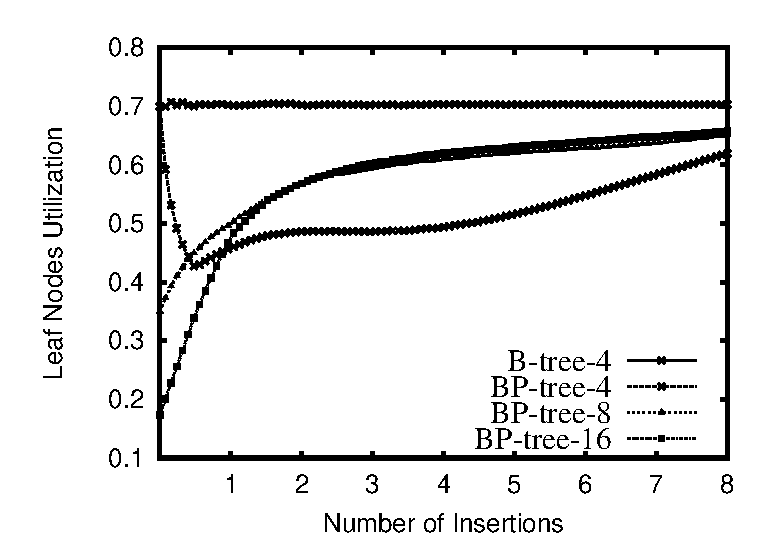
\includegraphics[scale = 0.65] {figs/zipf_result5.eps}

\caption{Leaf nodes utilization} \label{fig:exp:utilization}
\end{figure}

\subsection{Sensitivity to Data Distribution Changes}
In this section, we evaluate the sensitivity of our predictive
model to data distribution changes in order to show that our \bptree is stable
with the dataset of different data distributions. We change the dataset as
follows. The size of the dataset is 5 millions and the dataset follows
a skewed (Zipf) distribution. However, we gradually change the Zipf factors and
add a random offset every one million keys generated,
resulting in a change of the data distribution. We did
the insertion, update, search experiments as in previous sections.
In Figure~\ref{fig:exp:sensitivity}, we show comparisons of the
CPU cycles of all the four tree indexes with respect to different
operations.


From the figure, we can observe that the relative performance of
insertion, update and point search is very similar to that of the
previous experiments. For the leaf node utilization, when the node
size is 4 cache lines, the trend of the first half is similar to
that of the previous result, but the utilization decreases slightly
as the second half starts and increases again at last. The
reason of the decrease is that changes of data distribution caused
a wrong prediction from the predictive model and further caused
some improper splits. After that the predictive model adjusts its
prediction via the evaluation metrics and makes the structure
normal again which means that our evaluating scheme works fine 
and it can help the predictive model to modify the splitting strategy. 


We can also observe from Figure~\ref{fig:exp:sensitivity}(e) that
the stable utilization value is a bit smaller than that of the
previous experiments, which may have also caused the range search
performance to degrade slightly as shown in
Figure~\ref{fig:exp:sensitivity}(d). To summarize, the major
performance of the \bptree verified in the previous experiments
still holds when the data distribution changes which shows \bptree to be stable.

\begin{figure*}[!t]
\centering
\subfigure[Insertion]{
    \hspace*{-1.5em}\includegraphics[scale = 0.55] {figs/zipf_result921.eps}
    \label{fig:exp:sensitivity:subfig1}
} \subfigure[Update]{
    \hspace*{-1.5em}\includegraphics[scale = 0.55] {figs/zipf_result924.eps}
    \label{fig:exp:sensitivity:subfig2}
} \subfigure[Point Search]{
    \hspace*{-1.5em}\includegraphics[scale = 0.55] {figs/zipf_result922.eps}
    \label{fig:exp:sensitivity:subfig3}
} \subfigure[Range Search]{
    \hspace*{-1.5em}\includegraphics[scale = 0.55] {figs/zipf_result923.eps}
    \label{fig:exp:sensitivity:subfig4}
} \subfigure[Leaf Node Utilization]{
    \hspace*{-1.5em}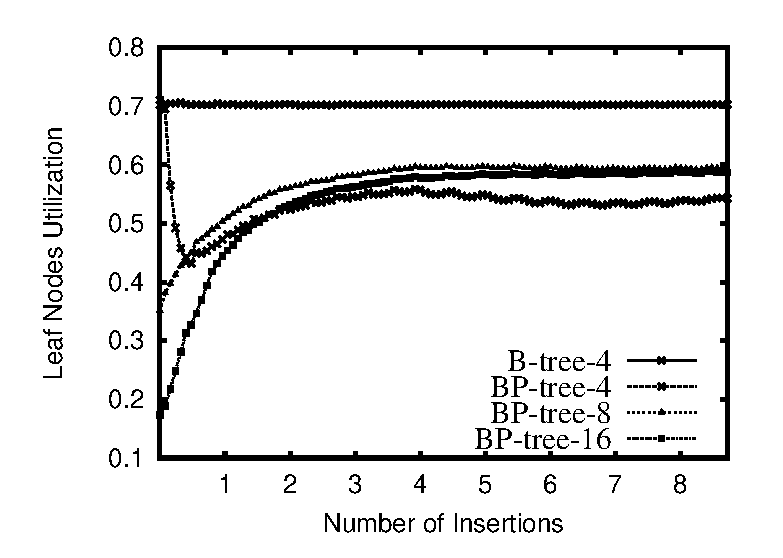
\includegraphics[scale = 0.55] {figs/zipf_result925.eps}
    \label{fig:exp:sensitivity:subfig5}
} \caption{Sensitivity to Data Distribution Changes}
\label{fig:exp:sensitivity}
\end{figure*}

\section{Summary}

In this chapter, we did an extensive experiments evaluation of our \bptree. We build our experimental
platform to simulate the PCM environment and compare it with some of the other write-optimized indexing
technique and the traditional normal \bplustree. We did the experiments based on both the uniform
dataset and skewed dataset. We observed that for both data distribution, our \bptree can work well.
The experimental results show that the \bptree significantly reduces
the number of writes for both the insertions and updates while having a good search performance at the same time,
therefore making it write and energy efficient and suitable for a PCM-like
hardware environment. The sensitivity experiments show that \bptree is a stable indexing technique and 
it works fine for different datasets. 


\newpage

\chapter{Conclusion}
\label{sec:conclusion}

In this chapter, we are going to conclude our work of this thesis and present a direction for the future work.

\section{Conclusion}

Phase change memory (PCM) is an emerging memory technology with many attractive features. In the near
future, PCM is expected to become a common component in the memory hierarchy of the computer systems.
On one hand, PCM could turn out to be a low-cost, more reliable, faster and better alternative to
flash memory. On the other hand, PCM is also a very promising alternative to the traditional DRAM to
become the major component of the main memory system.

However, PCM is still in its early stage and we still face some challenges to design algorithms for
PCM-based memory systems including the high read and write latency compared to DRAM, the limited lifetime
of the chip and the high energy consumption etc. If we want to make best use of PCM in the existing
systems, we need to overcome these challenges.

In this thesis, we proposed to study the algorithms redesigning for database systems on phase change memory, particularly
for indexing technique but in the future we can reconsider the whole technology stack of a traditional database systems.
In our work, we proposed the \bptree indexing structure to best take advantage of the good features of PCM.

The main design objective of our \bptree indexing is to
reduce the number of writes and energy consumption while keeping
the tree construction and search efficient. We developed a predictive model to
predict the near future data distribution based on the current data and then pre-allocate space for them in the
PCM memory to reduce the movements caused by node splits and merges.
We present the details of the model and show some metrics to
evaluate the performance of the model during the construction process.
If the metrics indicate that the prediction model is not running in a normal manner,
we will adjust the model or rebuild the index in the worst case.
The experiments on PostgreSQL database system showed
that our \bptree indexing scheme achieves a better performance than the traditional \bplustree and outperforms the state-of-the-art solution proposed in
\cite{chen2011rethinking}.
Additionally, our \bptree can be easily implemented in
existing commercial database systems based on the existing \bplustree structures.

\section{Future Work}

Database system is a very complex system and it consists of many complex subsystems\cite{ramakrishnan2003database,date1983introduction}. 
Currently we only considered the indexing technique but there are many others we can work on for example the query processing algorithms. 

In the future, we can continue to work on algorithms redesigning for PCM-based database systems. We can gradually move on the the query processing algorithms and buffer management. Since query processing is an important component of the database system, which will influence the overall performance of the whole system greatly, it needs to be redesigned carefully. 
%After that, I will implement the newly designed algorithms to the PostgreSQL system and finally what I want to do is that I implement both the indexing and query processing techniques into PostgreSQL and it can work efficiently without simulation when the PCM product comes out.
%Furthermore, our \bptree shows an idea about the indexing structure design for the other non-volatile memory with similar characteristics.
%In this section, we will briefly show some potential research problems and directions on query processing for PCM-based database systems that can be done in the near future. As we have shown in the previous Section~\ref{sec:technology}, the main design goal for algorithms for PCM-based database systems mainly lies in how to reduce the effect of the slow writes and further reduce the energy consumption and query latency.

In \cite{chen2011rethinking}, Chen, Gibbons and Nath have already done some work on hash joins. First they show the simple hash join, there are two phases, the build phase and the probe phase. In the build phase, the algorithm scans the smaller build relation and build a hash table for this relation. Then in the probe phase, the algorithm scans the larger probe relation. For each probe tuple, it computes the hash code and compare with the hash table to output the join result. The main disadvantage of the simple hash join is that whenever the size of the recode is large or not, it will lead to many cache misses, which can lead to a low performance. Then to solve the cache miss problem, the cache partitioning algorithm is introduced. The major difference is that in the build phase, instead of hashing the whole relation, the algorithm partitioned the two input relations using the same hash function so that every pair of the partitions can fit into the CPU cache. Then in the join phase, for each pair of the partition, the simple hash join algorithm can be used. The cache partitioning algorithm can solve the cache miss problem of the simple hash join. But it introduces a large number of writes which is not suitable for PCM-based database systems. Thus in this paper, the authors propose the virtual partitioning hash join, which is a variant of the cache partitioning method. The basic idea is that instead of physically copying input records into partitions, we perform the partitioning virtually. For each partition in build phase, we remember the record IDs and then in the join phase, we can use the record ID lists to join the records of a pair of partitions in place, thus avoiding the large number of writes in cache partitioning.

In our research, since we want to reduce the writes, we need to reconsider and redesign the operators if necessary, including scan, sort, join etc. Since PCM does not have the ``erase-before-write'' shortage, we do not need to focus on the erase and block writes. Since PCM supports fast random reads, we can work on the page layouts like the algorithms design for SSD to reduce the read latency. For refinement of operators, some of the existing techniques can be used like the ``first index and late materialization'' strategy which can reduce much writes.

Much work can be done for the query processing optimization for PCM-based database systems. In this thesis, we just show a direction and we can continue to work on this topic in the future.


\bibliography{thesis}
\newpage

\end{doublespacing}
\end{document}
